% Created by tikzDevice version 0.7.0 on 2014-06-29 16:56:16
% !TEX encoding = UTF-8 Unicode
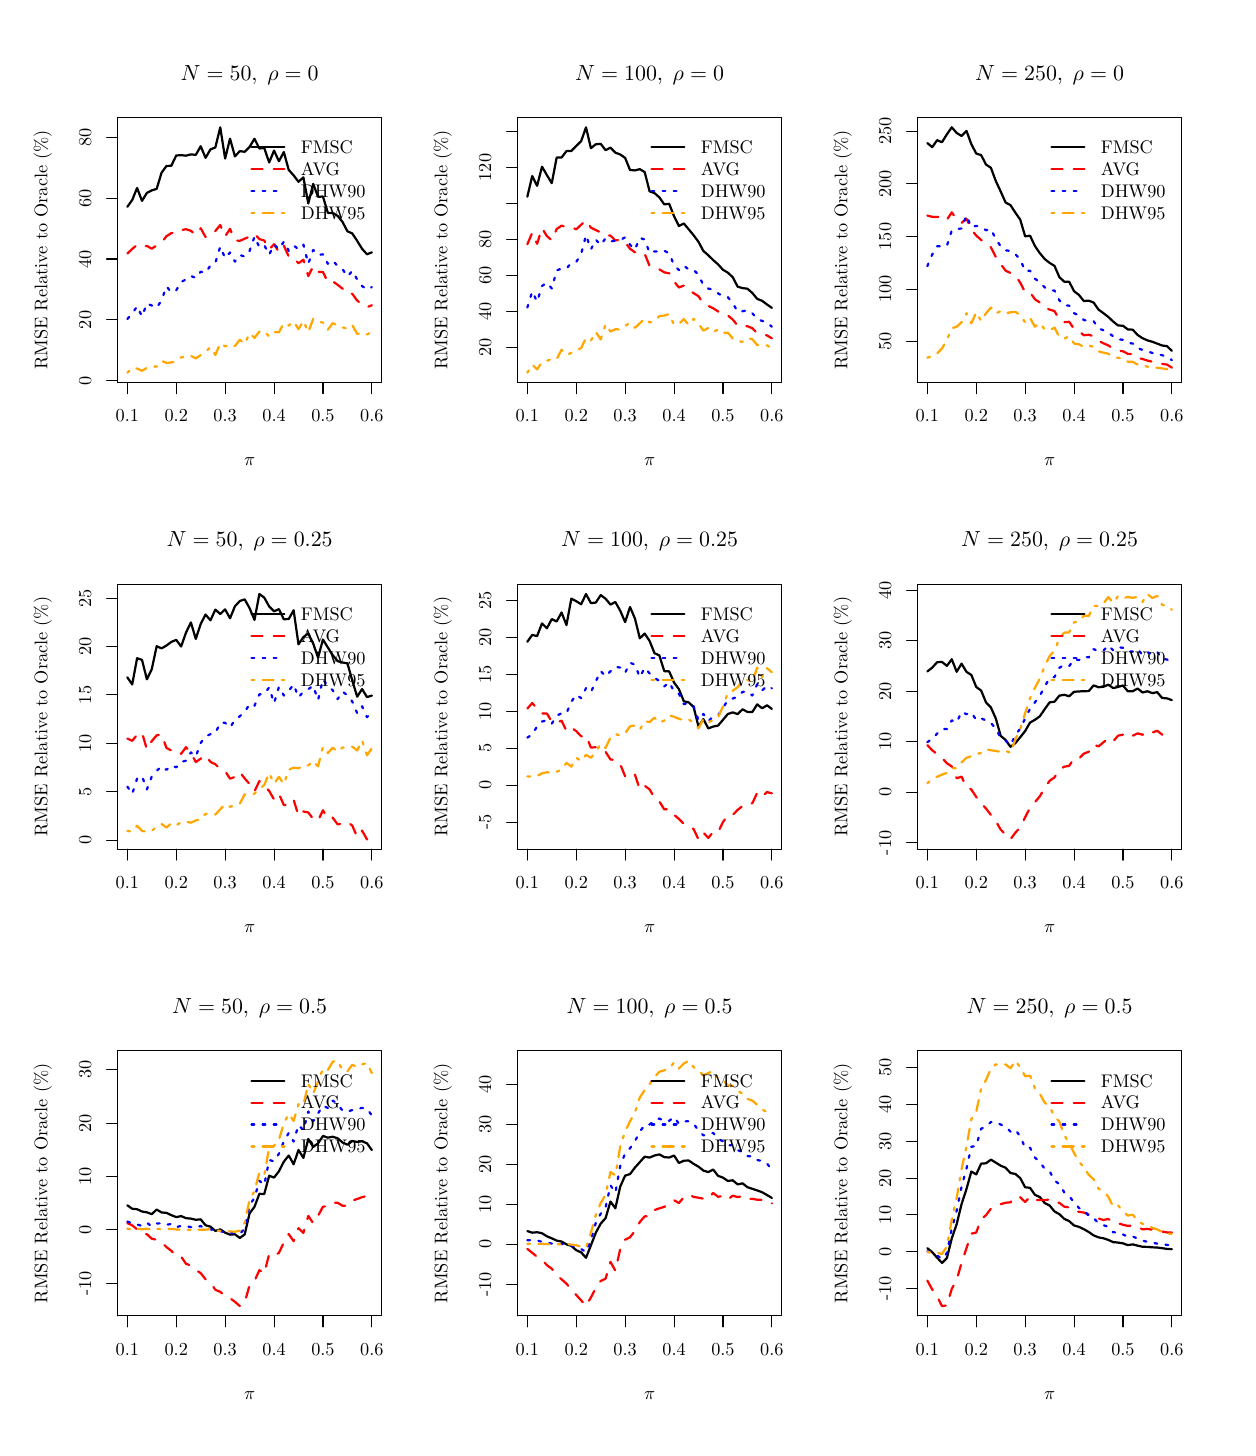
\begin{tikzpicture}[x=1pt,y=1pt]
\definecolor[named]{fillColor}{rgb}{1.00,1.00,1.00}
\path[use as bounding box,fill=fillColor,fill opacity=0.00] (0,0) rectangle (433.62,505.89);
\begin{scope}
\path[clip] ( 32.47,377.65) rectangle (127.91,473.42);
\definecolor[named]{drawColor}{rgb}{0.00,0.00,0.00}

\path[draw=drawColor,line width= 0.8pt,line join=round,line cap=round] ( 36.01,441.15) --
	( 37.77,443.61) --
	( 39.54,447.96) --
	( 41.31,443.30) --
	( 43.08,446.17) --
	( 44.84,447.09) --
	( 46.61,447.63) --
	( 48.38,453.47) --
	( 50.15,455.90) --
	( 51.91,456.00) --
	( 53.68,459.70) --
	( 55.45,459.82) --
	( 57.21,459.63) --
	( 58.98,460.10) --
	( 60.75,459.91) --
	( 62.52,463.04) --
	( 64.28,458.86) --
	( 66.05,461.90) --
	( 67.82,462.60) --
	( 69.59,469.87) --
	( 71.35,458.59) --
	( 73.12,465.79) --
	( 74.89,459.38) --
	( 76.66,461.27) --
	( 78.42,461.04) --
	( 80.19,462.81) --
	( 81.96,465.75) --
	( 83.72,462.23) --
	( 85.49,462.41) --
	( 87.26,457.19) --
	( 89.03,461.47) --
	( 90.79,457.62) --
	( 92.56,460.94) --
	( 94.33,454.48) --
	( 96.10,452.52) --
	( 97.86,450.19) --
	( 99.63,451.80) --
	(101.40,442.37) --
	(103.17,449.44) --
	(104.93,444.77) --
	(106.70,444.87) --
	(108.47,438.95) --
	(110.23,438.94) --
	(112.00,437.88) --
	(113.77,435.68) --
	(115.54,432.30) --
	(117.30,431.52) --
	(119.07,428.83) --
	(120.84,425.98) --
	(122.61,424.00) --
	(124.37,424.70);
\end{scope}
\begin{scope}
\path[clip] (  0.00,  0.00) rectangle (433.62,505.89);
\definecolor[named]{drawColor}{rgb}{0.00,0.00,0.00}

\path[draw=drawColor,line width= 0.4pt,line join=round,line cap=round] ( 36.01,377.65) -- (124.37,377.65);

\path[draw=drawColor,line width= 0.4pt,line join=round,line cap=round] ( 36.01,377.65) -- ( 36.01,373.69);

\path[draw=drawColor,line width= 0.4pt,line join=round,line cap=round] ( 53.68,377.65) -- ( 53.68,373.69);

\path[draw=drawColor,line width= 0.4pt,line join=round,line cap=round] ( 71.35,377.65) -- ( 71.35,373.69);

\path[draw=drawColor,line width= 0.4pt,line join=round,line cap=round] ( 89.03,377.65) -- ( 89.03,373.69);

\path[draw=drawColor,line width= 0.4pt,line join=round,line cap=round] (106.70,377.65) -- (106.70,373.69);

\path[draw=drawColor,line width= 0.4pt,line join=round,line cap=round] (124.37,377.65) -- (124.37,373.69);

\node[text=drawColor,anchor=base,inner sep=0pt, outer sep=0pt, scale=  0.66] at ( 36.01,363.40) {0.1};

\node[text=drawColor,anchor=base,inner sep=0pt, outer sep=0pt, scale=  0.66] at ( 53.68,363.40) {0.2};

\node[text=drawColor,anchor=base,inner sep=0pt, outer sep=0pt, scale=  0.66] at ( 71.35,363.40) {0.3};

\node[text=drawColor,anchor=base,inner sep=0pt, outer sep=0pt, scale=  0.66] at ( 89.03,363.40) {0.4};

\node[text=drawColor,anchor=base,inner sep=0pt, outer sep=0pt, scale=  0.66] at (106.70,363.40) {0.5};

\node[text=drawColor,anchor=base,inner sep=0pt, outer sep=0pt, scale=  0.66] at (124.37,363.40) {0.6};

\path[draw=drawColor,line width= 0.4pt,line join=round,line cap=round] ( 32.47,378.32) -- ( 32.47,466.24);

\path[draw=drawColor,line width= 0.4pt,line join=round,line cap=round] ( 32.47,378.32) -- ( 28.51,378.32);

\path[draw=drawColor,line width= 0.4pt,line join=round,line cap=round] ( 32.47,400.30) -- ( 28.51,400.30);

\path[draw=drawColor,line width= 0.4pt,line join=round,line cap=round] ( 32.47,422.28) -- ( 28.51,422.28);

\path[draw=drawColor,line width= 0.4pt,line join=round,line cap=round] ( 32.47,444.26) -- ( 28.51,444.26);

\path[draw=drawColor,line width= 0.4pt,line join=round,line cap=round] ( 32.47,466.24) -- ( 28.51,466.24);

\node[text=drawColor,rotate= 90.00,anchor=base,inner sep=0pt, outer sep=0pt, scale=  0.66] at ( 22.97,378.32) {0};

\node[text=drawColor,rotate= 90.00,anchor=base,inner sep=0pt, outer sep=0pt, scale=  0.66] at ( 22.97,400.30) {20};

\node[text=drawColor,rotate= 90.00,anchor=base,inner sep=0pt, outer sep=0pt, scale=  0.66] at ( 22.97,422.28) {40};

\node[text=drawColor,rotate= 90.00,anchor=base,inner sep=0pt, outer sep=0pt, scale=  0.66] at ( 22.97,444.26) {60};

\node[text=drawColor,rotate= 90.00,anchor=base,inner sep=0pt, outer sep=0pt, scale=  0.66] at ( 22.97,466.24) {80};

\path[draw=drawColor,line width= 0.4pt,line join=round,line cap=round] ( 32.47,377.65) --
	(127.91,377.65) --
	(127.91,473.42) --
	( 32.47,473.42) --
	( 32.47,377.65);
\end{scope}
\begin{scope}
\path[clip] (  0.00,337.26) rectangle (144.54,505.89);
\definecolor[named]{drawColor}{rgb}{0.00,0.00,0.00}

\node[text=drawColor,anchor=base,inner sep=0pt, outer sep=0pt, scale=  0.79] at ( 80.19,486.92) {\bfseries $N=50, \;\rho=0$};

\node[text=drawColor,anchor=base,inner sep=0pt, outer sep=0pt, scale=  0.66] at ( 80.19,347.56) {$\pi$};

\node[text=drawColor,rotate= 90.00,anchor=base,inner sep=0pt, outer sep=0pt, scale=  0.66] at (  7.13,425.53) {RMSE Relative to Oracle (\%)};
\end{scope}
\begin{scope}
\path[clip] ( 32.47,377.65) rectangle (127.91,473.42);
\definecolor[named]{drawColor}{rgb}{1.00,0.00,0.00}

\path[draw=drawColor,line width= 0.8pt,dash pattern=on 4pt off 4pt ,line join=round,line cap=round] ( 36.01,424.23) --
	( 37.77,425.92) --
	( 39.54,427.41) --
	( 41.31,426.78) --
	( 43.08,427.00) --
	( 44.84,426.03) --
	( 46.61,427.20) --
	( 48.38,428.24) --
	( 50.15,430.52) --
	( 51.91,431.65) --
	( 53.68,431.66) --
	( 55.45,432.72) --
	( 57.21,433.07) --
	( 58.98,432.48) --
	( 60.75,431.02) --
	( 62.52,433.39) --
	( 64.28,430.25) --
	( 66.05,431.49) --
	( 67.82,432.42) --
	( 69.59,434.58) --
	( 71.35,430.44) --
	( 73.12,433.18) --
	( 74.89,429.04) --
	( 76.66,428.85) --
	( 78.42,429.62) --
	( 80.19,430.41) --
	( 81.96,431.44) --
	( 83.72,429.50) --
	( 85.49,428.98) --
	( 87.26,425.71) --
	( 89.03,427.64) --
	( 90.79,424.77) --
	( 92.56,427.16) --
	( 94.33,423.17) --
	( 96.10,422.77) --
	( 97.86,420.75) --
	( 99.63,422.03) --
	(101.40,416.13) --
	(103.17,419.64) --
	(104.93,417.61) --
	(106.70,417.61) --
	(108.47,413.89) --
	(110.23,414.20) --
	(112.00,412.97) --
	(113.77,411.57) --
	(115.54,409.74) --
	(117.30,409.71) --
	(119.07,407.27) --
	(120.84,405.90) --
	(122.61,404.88) --
	(124.37,405.58);
\definecolor[named]{drawColor}{rgb}{0.00,0.00,1.00}

\path[draw=drawColor,line width= 0.8pt,dash pattern=on 1pt off 3pt ,line join=round,line cap=round] ( 36.01,400.61) --
	( 37.77,402.54) --
	( 39.54,405.21) --
	( 41.31,401.52) --
	( 43.08,406.21) --
	( 44.84,405.48) --
	( 46.61,404.64) --
	( 48.38,407.40) --
	( 50.15,412.38) --
	( 51.91,410.28) --
	( 53.68,411.00) --
	( 55.45,414.03) --
	( 57.21,414.87) --
	( 58.98,416.18) --
	( 60.75,415.42) --
	( 62.52,417.69) --
	( 64.28,417.31) --
	( 66.05,419.94) --
	( 67.82,420.90) --
	( 69.59,426.77) --
	( 71.35,422.60) --
	( 73.12,424.66) --
	( 74.89,421.36) --
	( 76.66,423.74) --
	( 78.42,423.18) --
	( 80.19,425.22) --
	( 81.96,430.35) --
	( 83.72,426.58) --
	( 85.49,427.29) --
	( 87.26,423.85) --
	( 89.03,427.50) --
	( 90.79,425.85) --
	( 92.56,428.56) --
	( 94.33,425.27) --
	( 96.10,427.19) --
	( 97.86,425.81) --
	( 99.63,427.49) --
	(101.40,420.59) --
	(103.17,425.57) --
	(104.93,423.74) --
	(106.70,423.98) --
	(108.47,420.58) --
	(110.23,421.80) --
	(112.00,419.69) --
	(113.77,418.64) --
	(115.54,415.94) --
	(117.30,418.01) --
	(119.07,414.89) --
	(120.84,412.50) --
	(122.61,411.28) --
	(124.37,412.12);
\definecolor[named]{drawColor}{rgb}{1.00,0.65,0.00}

\path[draw=drawColor,line width= 0.8pt,dash pattern=on 1pt off 3pt on 4pt off 3pt ,line join=round,line cap=round] ( 36.01,381.20) --
	( 37.77,382.92) --
	( 39.54,382.71) --
	( 41.31,381.90) --
	( 43.08,382.99) --
	( 44.84,383.40) --
	( 46.61,383.47) --
	( 48.38,385.47) --
	( 50.15,384.77) --
	( 51.91,384.89) --
	( 53.68,385.41) --
	( 55.45,386.73) --
	( 57.21,387.11) --
	( 58.98,387.30) --
	( 60.75,386.36) --
	( 62.52,387.57) --
	( 64.28,388.76) --
	( 66.05,390.44) --
	( 67.82,387.63) --
	( 69.59,391.84) --
	( 71.35,390.75) --
	( 73.12,391.37) --
	( 74.89,390.84) --
	( 76.66,393.11) --
	( 78.42,391.64) --
	( 80.19,395.51) --
	( 81.96,393.81) --
	( 83.72,396.06) --
	( 85.49,396.22) --
	( 87.26,394.29) --
	( 89.03,395.90) --
	( 90.79,395.81) --
	( 92.56,399.10) --
	( 94.33,398.23) --
	( 96.10,399.77) --
	( 97.86,396.94) --
	( 99.63,399.96) --
	(101.40,395.83) --
	(103.17,400.62) --
	(104.93,399.63) --
	(106.70,399.35) --
	(108.47,396.71) --
	(110.23,399.12) --
	(112.00,398.30) --
	(113.77,397.58) --
	(115.54,397.15) --
	(117.30,398.40) --
	(119.07,395.23) --
	(120.84,395.56) --
	(122.61,395.03) --
	(124.37,395.93);
\definecolor[named]{drawColor}{rgb}{0.00,0.00,0.00}

\path[draw=drawColor,line width= 0.8pt,line join=round,line cap=round] ( 80.89,462.63) -- ( 92.77,462.63);
\definecolor[named]{drawColor}{rgb}{1.00,0.00,0.00}

\path[draw=drawColor,line width= 0.8pt,dash pattern=on 4pt off 4pt ,line join=round,line cap=round] ( 80.89,454.71) -- ( 92.77,454.71);
\definecolor[named]{drawColor}{rgb}{0.00,0.00,1.00}

\path[draw=drawColor,line width= 0.8pt,dash pattern=on 1pt off 3pt ,line join=round,line cap=round] ( 80.89,446.79) -- ( 92.77,446.79);
\definecolor[named]{drawColor}{rgb}{1.00,0.65,0.00}

\path[draw=drawColor,line width= 0.8pt,dash pattern=on 1pt off 3pt on 4pt off 3pt ,line join=round,line cap=round] ( 80.89,438.87) -- ( 92.77,438.87);
\definecolor[named]{drawColor}{rgb}{0.00,0.00,0.00}

\node[text=drawColor,anchor=base west,inner sep=0pt, outer sep=0pt, scale=  0.66] at ( 98.71,460.35) {FMSC};

\node[text=drawColor,anchor=base west,inner sep=0pt, outer sep=0pt, scale=  0.66] at ( 98.71,452.43) {AVG};

\node[text=drawColor,anchor=base west,inner sep=0pt, outer sep=0pt, scale=  0.66] at ( 98.71,444.51) {DHW90};

\node[text=drawColor,anchor=base west,inner sep=0pt, outer sep=0pt, scale=  0.66] at ( 98.71,436.59) {DHW95};
\end{scope}
\begin{scope}
\path[clip] ( 32.47,209.02) rectangle (127.91,304.79);
\definecolor[named]{drawColor}{rgb}{0.00,0.00,0.00}

\path[draw=drawColor,line width= 0.8pt,line join=round,line cap=round] ( 36.01,271.15) --
	( 37.77,268.56) --
	( 39.54,278.04) --
	( 41.31,277.44) --
	( 43.08,270.40) --
	( 44.84,274.07) --
	( 46.61,282.37) --
	( 48.38,281.60) --
	( 50.15,282.61) --
	( 51.91,283.93) --
	( 53.68,284.66) --
	( 55.45,282.27) --
	( 57.21,287.30) --
	( 58.98,290.98) --
	( 60.75,285.01) --
	( 62.52,290.43) --
	( 64.28,293.81) --
	( 66.05,291.74) --
	( 67.82,295.60) --
	( 69.59,294.02) --
	( 71.35,295.69) --
	( 73.12,292.46) --
	( 74.89,296.80) --
	( 76.66,298.71) --
	( 78.42,299.30) --
	( 80.19,296.13) --
	( 81.96,291.86) --
	( 83.72,301.24) --
	( 85.49,299.94) --
	( 87.26,296.74) --
	( 89.03,294.99) --
	( 90.79,295.79) --
	( 92.56,292.12) --
	( 94.33,292.21) --
	( 96.10,295.36) --
	( 97.86,283.05) --
	( 99.63,285.66) --
	(101.40,287.00) --
	(103.17,283.32) --
	(104.93,278.26) --
	(106.70,284.79) --
	(108.47,281.92) --
	(110.23,279.14) --
	(112.00,276.98) --
	(113.77,276.49) --
	(115.54,276.19) --
	(117.30,269.97) --
	(119.07,264.14) --
	(120.84,266.90) --
	(122.61,264.00) --
	(124.37,264.52);
\end{scope}
\begin{scope}
\path[clip] (  0.00,  0.00) rectangle (433.62,505.89);
\definecolor[named]{drawColor}{rgb}{0.00,0.00,0.00}

\path[draw=drawColor,line width= 0.4pt,line join=round,line cap=round] ( 36.01,209.02) -- (124.37,209.02);

\path[draw=drawColor,line width= 0.4pt,line join=round,line cap=round] ( 36.01,209.02) -- ( 36.01,205.06);

\path[draw=drawColor,line width= 0.4pt,line join=round,line cap=round] ( 53.68,209.02) -- ( 53.68,205.06);

\path[draw=drawColor,line width= 0.4pt,line join=round,line cap=round] ( 71.35,209.02) -- ( 71.35,205.06);

\path[draw=drawColor,line width= 0.4pt,line join=round,line cap=round] ( 89.03,209.02) -- ( 89.03,205.06);

\path[draw=drawColor,line width= 0.4pt,line join=round,line cap=round] (106.70,209.02) -- (106.70,205.06);

\path[draw=drawColor,line width= 0.4pt,line join=round,line cap=round] (124.37,209.02) -- (124.37,205.06);

\node[text=drawColor,anchor=base,inner sep=0pt, outer sep=0pt, scale=  0.66] at ( 36.01,194.77) {0.1};

\node[text=drawColor,anchor=base,inner sep=0pt, outer sep=0pt, scale=  0.66] at ( 53.68,194.77) {0.2};

\node[text=drawColor,anchor=base,inner sep=0pt, outer sep=0pt, scale=  0.66] at ( 71.35,194.77) {0.3};

\node[text=drawColor,anchor=base,inner sep=0pt, outer sep=0pt, scale=  0.66] at ( 89.03,194.77) {0.4};

\node[text=drawColor,anchor=base,inner sep=0pt, outer sep=0pt, scale=  0.66] at (106.70,194.77) {0.5};

\node[text=drawColor,anchor=base,inner sep=0pt, outer sep=0pt, scale=  0.66] at (124.37,194.77) {0.6};

\path[draw=drawColor,line width= 0.4pt,line join=round,line cap=round] ( 32.47,212.33) -- ( 32.47,299.77);

\path[draw=drawColor,line width= 0.4pt,line join=round,line cap=round] ( 32.47,212.33) -- ( 28.51,212.33);

\path[draw=drawColor,line width= 0.4pt,line join=round,line cap=round] ( 32.47,229.82) -- ( 28.51,229.82);

\path[draw=drawColor,line width= 0.4pt,line join=round,line cap=round] ( 32.47,247.30) -- ( 28.51,247.30);

\path[draw=drawColor,line width= 0.4pt,line join=round,line cap=round] ( 32.47,264.79) -- ( 28.51,264.79);

\path[draw=drawColor,line width= 0.4pt,line join=round,line cap=round] ( 32.47,282.28) -- ( 28.51,282.28);

\path[draw=drawColor,line width= 0.4pt,line join=round,line cap=round] ( 32.47,299.77) -- ( 28.51,299.77);

\node[text=drawColor,rotate= 90.00,anchor=base,inner sep=0pt, outer sep=0pt, scale=  0.66] at ( 22.97,212.33) {0};

\node[text=drawColor,rotate= 90.00,anchor=base,inner sep=0pt, outer sep=0pt, scale=  0.66] at ( 22.97,229.82) {5};

\node[text=drawColor,rotate= 90.00,anchor=base,inner sep=0pt, outer sep=0pt, scale=  0.66] at ( 22.97,247.30) {10};

\node[text=drawColor,rotate= 90.00,anchor=base,inner sep=0pt, outer sep=0pt, scale=  0.66] at ( 22.97,264.79) {15};

\node[text=drawColor,rotate= 90.00,anchor=base,inner sep=0pt, outer sep=0pt, scale=  0.66] at ( 22.97,282.28) {20};

\node[text=drawColor,rotate= 90.00,anchor=base,inner sep=0pt, outer sep=0pt, scale=  0.66] at ( 22.97,299.77) {25};

\path[draw=drawColor,line width= 0.4pt,line join=round,line cap=round] ( 32.47,209.02) --
	(127.91,209.02) --
	(127.91,304.79) --
	( 32.47,304.79) --
	( 32.47,209.02);
\end{scope}
\begin{scope}
\path[clip] (  0.00,168.63) rectangle (144.54,337.26);
\definecolor[named]{drawColor}{rgb}{0.00,0.00,0.00}

\node[text=drawColor,anchor=base,inner sep=0pt, outer sep=0pt, scale=  0.79] at ( 80.19,318.29) {\bfseries $N=50, \;\rho=0.25$};

\node[text=drawColor,anchor=base,inner sep=0pt, outer sep=0pt, scale=  0.66] at ( 80.19,178.93) {$\pi$};

\node[text=drawColor,rotate= 90.00,anchor=base,inner sep=0pt, outer sep=0pt, scale=  0.66] at (  7.13,256.90) {RMSE Relative to Oracle (\%)};
\end{scope}
\begin{scope}
\path[clip] ( 32.47,209.02) rectangle (127.91,304.79);
\definecolor[named]{drawColor}{rgb}{1.00,0.00,0.00}

\path[draw=drawColor,line width= 0.8pt,dash pattern=on 4pt off 4pt ,line join=round,line cap=round] ( 36.01,249.01) --
	( 37.77,248.19) --
	( 39.54,250.36) --
	( 41.31,251.16) --
	( 43.08,245.09) --
	( 44.84,248.09) --
	( 46.61,250.16) --
	( 48.38,250.52) --
	( 50.15,245.62) --
	( 51.91,244.70) --
	( 53.68,244.86) --
	( 55.45,243.49) --
	( 57.21,245.88) --
	( 58.98,243.75) --
	( 60.75,240.53) --
	( 62.52,241.75) --
	( 64.28,242.95) --
	( 66.05,240.56) --
	( 67.82,239.72) --
	( 69.59,238.03) --
	( 71.35,237.25) --
	( 73.12,234.50) --
	( 74.89,235.14) --
	( 76.66,236.88) --
	( 78.42,234.59) --
	( 80.19,232.56) --
	( 81.96,229.93) --
	( 83.72,233.64) --
	( 85.49,231.90) --
	( 87.26,230.09) --
	( 89.03,227.01) --
	( 90.79,229.03) --
	( 92.56,224.99) --
	( 94.33,225.11) --
	( 96.10,226.91) --
	( 97.86,221.12) --
	( 99.63,222.66) --
	(101.40,222.30) --
	(103.17,219.98) --
	(104.93,219.33) --
	(106.70,223.10) --
	(108.47,220.11) --
	(110.23,220.41) --
	(112.00,218.01) --
	(113.77,218.33) --
	(115.54,218.85) --
	(117.30,217.55) --
	(119.07,213.45) --
	(120.84,215.73) --
	(122.61,212.57) --
	(124.37,216.07);
\definecolor[named]{drawColor}{rgb}{0.00,0.00,1.00}

\path[draw=drawColor,line width= 0.8pt,dash pattern=on 1pt off 3pt ,line join=round,line cap=round] ( 36.01,231.65) --
	( 37.77,229.00) --
	( 39.54,234.53) --
	( 41.31,235.44) --
	( 43.08,230.63) --
	( 44.84,235.28) --
	( 46.61,237.35) --
	( 48.38,239.00) --
	( 50.15,237.70) --
	( 51.91,239.21) --
	( 53.68,238.63) --
	( 55.45,240.57) --
	( 57.21,241.00) --
	( 58.98,244.01) --
	( 60.75,242.52) --
	( 62.52,247.46) --
	( 64.28,249.72) --
	( 66.05,250.60) --
	( 67.82,251.00) --
	( 69.59,254.68) --
	( 71.35,254.72) --
	( 73.12,253.05) --
	( 74.89,255.70) --
	( 76.66,257.08) --
	( 78.42,258.58) --
	( 80.19,261.48) --
	( 81.96,260.85) --
	( 83.72,264.98) --
	( 85.49,265.20) --
	( 87.26,267.46) --
	( 89.03,261.81) --
	( 90.79,267.68) --
	( 92.56,264.58) --
	( 94.33,266.27) --
	( 96.10,268.56) --
	( 97.86,263.88) --
	( 99.63,265.93) --
	(101.40,266.87) --
	(103.17,268.09) --
	(104.93,262.93) --
	(106.70,270.44) --
	(108.47,267.89) --
	(110.23,266.48) --
	(112.00,263.26) --
	(113.77,265.98) --
	(115.54,264.64) --
	(117.30,262.37) --
	(119.07,258.15) --
	(120.84,260.66) --
	(122.61,256.74) --
	(124.37,258.53);
\definecolor[named]{drawColor}{rgb}{1.00,0.65,0.00}

\path[draw=drawColor,line width= 0.8pt,dash pattern=on 1pt off 3pt on 4pt off 3pt ,line join=round,line cap=round] ( 36.01,215.63) --
	( 37.77,215.43) --
	( 39.54,217.49) --
	( 41.31,215.66) --
	( 43.08,215.30) --
	( 44.84,215.61) --
	( 46.61,217.24) --
	( 48.38,218.15) --
	( 50.15,216.86) --
	( 51.91,218.38) --
	( 53.68,217.61) --
	( 55.45,218.82) --
	( 57.21,218.95) --
	( 58.98,218.61) --
	( 60.75,219.42) --
	( 62.52,219.83) --
	( 64.28,221.80) --
	( 66.05,221.76) --
	( 67.82,221.56) --
	( 69.59,223.44) --
	( 71.35,225.27) --
	( 73.12,224.37) --
	( 74.89,224.90) --
	( 76.66,225.51) --
	( 78.42,228.84) --
	( 80.19,228.59) --
	( 81.96,229.14) --
	( 83.72,230.79) --
	( 85.49,232.20) --
	( 87.26,236.58) --
	( 89.03,232.72) --
	( 90.79,235.17) --
	( 92.56,232.54) --
	( 94.33,237.71) --
	( 96.10,238.51) --
	( 97.86,238.24) --
	( 99.63,239.16) --
	(101.40,239.30) --
	(103.17,240.87) --
	(104.93,238.95) --
	(106.70,246.06) --
	(108.47,243.80) --
	(110.23,245.72) --
	(112.00,244.23) --
	(113.77,245.76) --
	(115.54,245.75) --
	(117.30,246.07) --
	(119.07,244.70) --
	(120.84,248.35) --
	(122.61,242.93) --
	(124.37,245.51);
\definecolor[named]{drawColor}{rgb}{0.00,0.00,0.00}

\path[draw=drawColor,line width= 0.8pt,line join=round,line cap=round] ( 80.89,294.00) -- ( 92.77,294.00);
\definecolor[named]{drawColor}{rgb}{1.00,0.00,0.00}

\path[draw=drawColor,line width= 0.8pt,dash pattern=on 4pt off 4pt ,line join=round,line cap=round] ( 80.89,286.08) -- ( 92.77,286.08);
\definecolor[named]{drawColor}{rgb}{0.00,0.00,1.00}

\path[draw=drawColor,line width= 0.8pt,dash pattern=on 1pt off 3pt ,line join=round,line cap=round] ( 80.89,278.16) -- ( 92.77,278.16);
\definecolor[named]{drawColor}{rgb}{1.00,0.65,0.00}

\path[draw=drawColor,line width= 0.8pt,dash pattern=on 1pt off 3pt on 4pt off 3pt ,line join=round,line cap=round] ( 80.89,270.24) -- ( 92.77,270.24);
\definecolor[named]{drawColor}{rgb}{0.00,0.00,0.00}

\node[text=drawColor,anchor=base west,inner sep=0pt, outer sep=0pt, scale=  0.66] at ( 98.71,291.72) {FMSC};

\node[text=drawColor,anchor=base west,inner sep=0pt, outer sep=0pt, scale=  0.66] at ( 98.71,283.80) {AVG};

\node[text=drawColor,anchor=base west,inner sep=0pt, outer sep=0pt, scale=  0.66] at ( 98.71,275.88) {DHW90};

\node[text=drawColor,anchor=base west,inner sep=0pt, outer sep=0pt, scale=  0.66] at ( 98.71,267.96) {DHW95};
\end{scope}
\begin{scope}
\path[clip] ( 32.47, 40.39) rectangle (127.91,136.16);
\definecolor[named]{drawColor}{rgb}{0.00,0.00,0.00}

\path[draw=drawColor,line width= 0.8pt,line join=round,line cap=round] ( 36.01, 80.35) --
	( 37.77, 79.10) --
	( 39.54, 78.94) --
	( 41.31, 78.11) --
	( 43.08, 77.81) --
	( 44.84, 77.15) --
	( 46.61, 78.82) --
	( 48.38, 77.76) --
	( 50.15, 77.62) --
	( 51.91, 76.79) --
	( 53.68, 76.08) --
	( 55.45, 76.46) --
	( 57.21, 75.70) --
	( 58.98, 75.54) --
	( 60.75, 75.12) --
	( 62.52, 75.28) --
	( 64.28, 73.13) --
	( 66.05, 72.64) --
	( 67.82, 71.10) --
	( 69.59, 71.65) --
	( 71.35, 70.47) --
	( 73.12, 69.74) --
	( 74.89, 69.88) --
	( 76.66, 68.56) --
	( 78.42, 69.84) --
	( 80.19, 77.45) --
	( 81.96, 79.82) --
	( 83.72, 84.50) --
	( 85.49, 84.44) --
	( 87.26, 91.03) --
	( 89.03, 90.38) --
	( 90.79, 92.63) --
	( 92.56, 96.13) --
	( 94.33, 98.35) --
	( 96.10, 95.18) --
	( 97.86,100.36) --
	( 99.63, 97.49) --
	(101.40,104.30) --
	(103.17,101.45) --
	(104.93,102.74) --
	(106.70,105.41) --
	(108.47,104.79) --
	(110.23,105.13) --
	(112.00,104.58) --
	(113.77,103.05) --
	(115.54,102.25) --
	(117.30,103.57) --
	(119.07,103.25) --
	(120.84,103.50) --
	(122.61,102.75) --
	(124.37,100.32);
\end{scope}
\begin{scope}
\path[clip] (  0.00,  0.00) rectangle (433.62,505.89);
\definecolor[named]{drawColor}{rgb}{0.00,0.00,0.00}

\path[draw=drawColor,line width= 0.4pt,line join=round,line cap=round] ( 36.01, 40.39) -- (124.37, 40.39);

\path[draw=drawColor,line width= 0.4pt,line join=round,line cap=round] ( 36.01, 40.39) -- ( 36.01, 36.43);

\path[draw=drawColor,line width= 0.4pt,line join=round,line cap=round] ( 53.68, 40.39) -- ( 53.68, 36.43);

\path[draw=drawColor,line width= 0.4pt,line join=round,line cap=round] ( 71.35, 40.39) -- ( 71.35, 36.43);

\path[draw=drawColor,line width= 0.4pt,line join=round,line cap=round] ( 89.03, 40.39) -- ( 89.03, 36.43);

\path[draw=drawColor,line width= 0.4pt,line join=round,line cap=round] (106.70, 40.39) -- (106.70, 36.43);

\path[draw=drawColor,line width= 0.4pt,line join=round,line cap=round] (124.37, 40.39) -- (124.37, 36.43);

\node[text=drawColor,anchor=base,inner sep=0pt, outer sep=0pt, scale=  0.66] at ( 36.01, 26.14) {0.1};

\node[text=drawColor,anchor=base,inner sep=0pt, outer sep=0pt, scale=  0.66] at ( 53.68, 26.14) {0.2};

\node[text=drawColor,anchor=base,inner sep=0pt, outer sep=0pt, scale=  0.66] at ( 71.35, 26.14) {0.3};

\node[text=drawColor,anchor=base,inner sep=0pt, outer sep=0pt, scale=  0.66] at ( 89.03, 26.14) {0.4};

\node[text=drawColor,anchor=base,inner sep=0pt, outer sep=0pt, scale=  0.66] at (106.70, 26.14) {0.5};

\node[text=drawColor,anchor=base,inner sep=0pt, outer sep=0pt, scale=  0.66] at (124.37, 26.14) {0.6};

\path[draw=drawColor,line width= 0.4pt,line join=round,line cap=round] ( 32.47, 52.18) -- ( 32.47,129.32);

\path[draw=drawColor,line width= 0.4pt,line join=round,line cap=round] ( 32.47, 52.18) -- ( 28.51, 52.18);

\path[draw=drawColor,line width= 0.4pt,line join=round,line cap=round] ( 32.47, 71.46) -- ( 28.51, 71.46);

\path[draw=drawColor,line width= 0.4pt,line join=round,line cap=round] ( 32.47, 90.75) -- ( 28.51, 90.75);

\path[draw=drawColor,line width= 0.4pt,line join=round,line cap=round] ( 32.47,110.03) -- ( 28.51,110.03);

\path[draw=drawColor,line width= 0.4pt,line join=round,line cap=round] ( 32.47,129.32) -- ( 28.51,129.32);

\node[text=drawColor,rotate= 90.00,anchor=base,inner sep=0pt, outer sep=0pt, scale=  0.66] at ( 22.97, 52.18) {-10};

\node[text=drawColor,rotate= 90.00,anchor=base,inner sep=0pt, outer sep=0pt, scale=  0.66] at ( 22.97, 71.46) {0};

\node[text=drawColor,rotate= 90.00,anchor=base,inner sep=0pt, outer sep=0pt, scale=  0.66] at ( 22.97, 90.75) {10};

\node[text=drawColor,rotate= 90.00,anchor=base,inner sep=0pt, outer sep=0pt, scale=  0.66] at ( 22.97,110.03) {20};

\node[text=drawColor,rotate= 90.00,anchor=base,inner sep=0pt, outer sep=0pt, scale=  0.66] at ( 22.97,129.32) {30};

\path[draw=drawColor,line width= 0.4pt,line join=round,line cap=round] ( 32.47, 40.39) --
	(127.91, 40.39) --
	(127.91,136.16) --
	( 32.47,136.16) --
	( 32.47, 40.39);
\end{scope}
\begin{scope}
\path[clip] (  0.00,  0.00) rectangle (144.54,168.63);
\definecolor[named]{drawColor}{rgb}{0.00,0.00,0.00}

\node[text=drawColor,anchor=base,inner sep=0pt, outer sep=0pt, scale=  0.79] at ( 80.19,149.66) {\bfseries $N=50, \;\rho=0.5$};

\node[text=drawColor,anchor=base,inner sep=0pt, outer sep=0pt, scale=  0.66] at ( 80.19, 10.30) {$\pi$};

\node[text=drawColor,rotate= 90.00,anchor=base,inner sep=0pt, outer sep=0pt, scale=  0.66] at (  7.13, 88.27) {RMSE Relative to Oracle (\%)};
\end{scope}
\begin{scope}
\path[clip] ( 32.47, 40.39) rectangle (127.91,136.16);
\definecolor[named]{drawColor}{rgb}{1.00,0.00,0.00}

\path[draw=drawColor,line width= 0.8pt,dash pattern=on 4pt off 4pt ,line join=round,line cap=round] ( 36.01, 73.92) --
	( 37.77, 73.10) --
	( 39.54, 71.70) --
	( 41.31, 70.18) --
	( 43.08, 69.90) --
	( 44.84, 68.29) --
	( 46.61, 67.90) --
	( 48.38, 67.05) --
	( 50.15, 65.24) --
	( 51.91, 63.91) --
	( 53.68, 61.96) --
	( 55.45, 61.81) --
	( 57.21, 59.23) --
	( 58.98, 58.57) --
	( 60.75, 56.99) --
	( 62.52, 55.84) --
	( 64.28, 53.63) --
	( 66.05, 52.42) --
	( 67.82, 49.81) --
	( 69.59, 49.08) --
	( 71.35, 47.56) --
	( 73.12, 46.79) --
	( 74.89, 45.49) --
	( 76.66, 43.94) --
	( 78.42, 45.17) --
	( 80.19, 51.52) --
	( 81.96, 52.98) --
	( 83.72, 56.91) --
	( 85.49, 55.69) --
	( 87.26, 62.73) --
	( 89.03, 62.16) --
	( 90.79, 63.17) --
	( 92.56, 66.90) --
	( 94.33, 69.97) --
	( 96.10, 67.39) --
	( 97.86, 72.07) --
	( 99.63, 70.39) --
	(101.40, 76.51) --
	(103.17, 73.90) --
	(104.93, 76.57) --
	(106.70, 79.83) --
	(108.47, 80.10) --
	(110.23, 81.26) --
	(112.00, 81.27) --
	(113.77, 80.17) --
	(115.54, 80.27) --
	(117.30, 82.08) --
	(119.07, 82.63) --
	(120.84, 83.31) --
	(122.61, 83.71) --
	(124.37, 82.08);
\definecolor[named]{drawColor}{rgb}{0.00,0.00,1.00}

\path[draw=drawColor,line width= 0.8pt,dash pattern=on 1pt off 3pt ,line join=round,line cap=round] ( 36.01, 74.48) --
	( 37.77, 73.89) --
	( 39.54, 73.43) --
	( 41.31, 72.88) --
	( 43.08, 74.04) --
	( 44.84, 72.72) --
	( 46.61, 73.80) --
	( 48.38, 73.84) --
	( 50.15, 73.31) --
	( 51.91, 73.62) --
	( 53.68, 72.42) --
	( 55.45, 72.96) --
	( 57.21, 72.81) --
	( 58.98, 72.46) --
	( 60.75, 72.29) --
	( 62.52, 72.87) --
	( 64.28, 71.88) --
	( 66.05, 71.76) --
	( 67.82, 70.92) --
	( 69.59, 71.03) --
	( 71.35, 70.53) --
	( 73.12, 70.42) --
	( 74.89, 70.30) --
	( 76.66, 69.99) --
	( 78.42, 71.99) --
	( 80.19, 80.44) --
	( 81.96, 83.01) --
	( 83.72, 89.23) --
	( 85.49, 87.68) --
	( 87.26, 96.71) --
	( 89.03, 96.25) --
	( 90.79, 99.00) --
	( 92.56,103.42) --
	( 94.33,106.51) --
	( 96.10,103.39) --
	( 97.86,109.38) --
	( 99.63,107.48) --
	(101.40,114.24) --
	(103.17,110.73) --
	(104.93,113.59) --
	(106.70,116.31) --
	(108.47,115.53) --
	(110.23,118.19) --
	(112.00,117.03) --
	(113.77,114.50) --
	(115.54,114.18) --
	(117.30,114.78) --
	(119.07,115.27) --
	(120.84,115.53) --
	(122.61,115.33) --
	(124.37,112.76);
\definecolor[named]{drawColor}{rgb}{1.00,0.65,0.00}

\path[draw=drawColor,line width= 0.8pt,dash pattern=on 1pt off 3pt on 4pt off 3pt ,line join=round,line cap=round] ( 36.01, 71.88) --
	( 37.77, 71.68) --
	( 39.54, 71.90) --
	( 41.31, 71.68) --
	( 43.08, 71.89) --
	( 44.84, 71.44) --
	( 46.61, 71.80) --
	( 48.38, 71.78) --
	( 50.15, 71.87) --
	( 51.91, 71.80) --
	( 53.68, 71.64) --
	( 55.45, 71.47) --
	( 57.21, 71.63) --
	( 58.98, 71.40) --
	( 60.75, 71.68) --
	( 62.52, 71.47) --
	( 64.28, 71.57) --
	( 66.05, 71.76) --
	( 67.82, 71.48) --
	( 69.59, 71.06) --
	( 71.35, 71.19) --
	( 73.12, 70.91) --
	( 74.89, 70.79) --
	( 76.66, 71.21) --
	( 78.42, 74.09) --
	( 80.19, 82.43) --
	( 81.96, 85.43) --
	( 83.72, 92.28) --
	( 85.49, 91.28) --
	( 87.26,101.25) --
	( 89.03,101.87) --
	( 90.79,103.96) --
	( 92.56,109.93) --
	( 94.33,113.42) --
	( 96.10,110.82) --
	( 97.86,116.90) --
	( 99.63,116.59) --
	(101.40,124.26) --
	(103.17,120.78) --
	(104.93,125.05) --
	(106.70,129.73) --
	(108.47,129.19) --
	(110.23,132.26) --
	(112.00,132.61) --
	(113.77,129.11) --
	(115.54,128.77) --
	(117.30,131.14) --
	(119.07,130.29) --
	(120.84,131.29) --
	(122.61,131.75) --
	(124.37,128.13);
\definecolor[named]{drawColor}{rgb}{0.00,0.00,0.00}

\path[draw=drawColor,line width= 0.8pt,line join=round,line cap=round] ( 80.89,125.37) -- ( 92.77,125.37);
\definecolor[named]{drawColor}{rgb}{1.00,0.00,0.00}

\path[draw=drawColor,line width= 0.8pt,dash pattern=on 4pt off 4pt ,line join=round,line cap=round] ( 80.89,117.45) -- ( 92.77,117.45);
\definecolor[named]{drawColor}{rgb}{0.00,0.00,1.00}

\path[draw=drawColor,line width= 0.8pt,dash pattern=on 1pt off 3pt ,line join=round,line cap=round] ( 80.89,109.53) -- ( 92.77,109.53);
\definecolor[named]{drawColor}{rgb}{1.00,0.65,0.00}

\path[draw=drawColor,line width= 0.8pt,dash pattern=on 1pt off 3pt on 4pt off 3pt ,line join=round,line cap=round] ( 80.89,101.61) -- ( 92.77,101.61);
\definecolor[named]{drawColor}{rgb}{0.00,0.00,0.00}

\node[text=drawColor,anchor=base west,inner sep=0pt, outer sep=0pt, scale=  0.66] at ( 98.71,123.09) {FMSC};

\node[text=drawColor,anchor=base west,inner sep=0pt, outer sep=0pt, scale=  0.66] at ( 98.71,115.17) {AVG};

\node[text=drawColor,anchor=base west,inner sep=0pt, outer sep=0pt, scale=  0.66] at ( 98.71,107.25) {DHW90};

\node[text=drawColor,anchor=base west,inner sep=0pt, outer sep=0pt, scale=  0.66] at ( 98.71, 99.33) {DHW95};
\end{scope}
\begin{scope}
\path[clip] (177.01,377.65) rectangle (272.45,473.42);
\definecolor[named]{drawColor}{rgb}{0.00,0.00,0.00}

\path[draw=drawColor,line width= 0.8pt,line join=round,line cap=round] (180.55,444.80) --
	(182.31,452.26) --
	(184.08,448.74) --
	(185.85,455.65) --
	(187.62,452.61) --
	(189.38,449.69) --
	(191.15,458.96) --
	(192.92,458.95) --
	(194.69,461.29) --
	(196.45,461.32) --
	(198.22,463.15) --
	(199.99,464.86) --
	(201.75,469.87) --
	(203.52,462.34) --
	(205.29,463.75) --
	(207.06,463.90) --
	(208.82,461.63) --
	(210.59,462.54) --
	(212.36,460.71) --
	(214.13,460.06) --
	(215.89,458.82) --
	(217.66,454.46) --
	(219.43,454.30) --
	(221.20,454.76) --
	(222.96,453.70) --
	(224.73,446.74) --
	(226.50,446.10) --
	(228.26,444.56) --
	(230.03,442.03) --
	(231.80,442.24) --
	(233.57,437.75) --
	(235.33,434.22) --
	(237.10,435.13) --
	(238.87,433.01) --
	(240.64,430.88) --
	(242.40,428.49) --
	(244.17,425.19) --
	(245.94,423.65) --
	(247.71,421.89) --
	(249.47,420.36) --
	(251.24,418.41) --
	(253.01,417.36) --
	(254.77,415.72) --
	(256.54,412.30) --
	(258.31,411.78) --
	(260.08,411.56) --
	(261.84,410.02) --
	(263.61,407.89) --
	(265.38,407.18) --
	(267.15,405.87) --
	(268.91,404.63);
\end{scope}
\begin{scope}
\path[clip] (  0.00,  0.00) rectangle (433.62,505.89);
\definecolor[named]{drawColor}{rgb}{0.00,0.00,0.00}

\path[draw=drawColor,line width= 0.4pt,line join=round,line cap=round] (180.55,377.65) -- (268.91,377.65);

\path[draw=drawColor,line width= 0.4pt,line join=round,line cap=round] (180.55,377.65) -- (180.55,373.69);

\path[draw=drawColor,line width= 0.4pt,line join=round,line cap=round] (198.22,377.65) -- (198.22,373.69);

\path[draw=drawColor,line width= 0.4pt,line join=round,line cap=round] (215.89,377.65) -- (215.89,373.69);

\path[draw=drawColor,line width= 0.4pt,line join=round,line cap=round] (233.57,377.65) -- (233.57,373.69);

\path[draw=drawColor,line width= 0.4pt,line join=round,line cap=round] (251.24,377.65) -- (251.24,373.69);

\path[draw=drawColor,line width= 0.4pt,line join=round,line cap=round] (268.91,377.65) -- (268.91,373.69);

\node[text=drawColor,anchor=base,inner sep=0pt, outer sep=0pt, scale=  0.66] at (180.55,363.40) {0.1};

\node[text=drawColor,anchor=base,inner sep=0pt, outer sep=0pt, scale=  0.66] at (198.22,363.40) {0.2};

\node[text=drawColor,anchor=base,inner sep=0pt, outer sep=0pt, scale=  0.66] at (215.89,363.40) {0.3};

\node[text=drawColor,anchor=base,inner sep=0pt, outer sep=0pt, scale=  0.66] at (233.57,363.40) {0.4};

\node[text=drawColor,anchor=base,inner sep=0pt, outer sep=0pt, scale=  0.66] at (251.24,363.40) {0.5};

\node[text=drawColor,anchor=base,inner sep=0pt, outer sep=0pt, scale=  0.66] at (268.91,363.40) {0.6};

\path[draw=drawColor,line width= 0.4pt,line join=round,line cap=round] (177.01,390.41) -- (177.01,468.34);

\path[draw=drawColor,line width= 0.4pt,line join=round,line cap=round] (177.01,390.41) -- (173.05,390.41);

\path[draw=drawColor,line width= 0.4pt,line join=round,line cap=round] (177.01,403.40) -- (173.05,403.40);

\path[draw=drawColor,line width= 0.4pt,line join=round,line cap=round] (177.01,416.39) -- (173.05,416.39);

\path[draw=drawColor,line width= 0.4pt,line join=round,line cap=round] (177.01,429.38) -- (173.05,429.38);

\path[draw=drawColor,line width= 0.4pt,line join=round,line cap=round] (177.01,442.36) -- (173.05,442.36);

\path[draw=drawColor,line width= 0.4pt,line join=round,line cap=round] (177.01,455.35) -- (173.05,455.35);

\path[draw=drawColor,line width= 0.4pt,line join=round,line cap=round] (177.01,468.34) -- (173.05,468.34);

\node[text=drawColor,rotate= 90.00,anchor=base,inner sep=0pt, outer sep=0pt, scale=  0.66] at (167.51,390.41) {20};

\node[text=drawColor,rotate= 90.00,anchor=base,inner sep=0pt, outer sep=0pt, scale=  0.66] at (167.51,403.40) {40};

\node[text=drawColor,rotate= 90.00,anchor=base,inner sep=0pt, outer sep=0pt, scale=  0.66] at (167.51,416.39) {60};

\node[text=drawColor,rotate= 90.00,anchor=base,inner sep=0pt, outer sep=0pt, scale=  0.66] at (167.51,429.38) {80};

\node[text=drawColor,rotate= 90.00,anchor=base,inner sep=0pt, outer sep=0pt, scale=  0.66] at (167.51,455.35) {120};

\path[draw=drawColor,line width= 0.4pt,line join=round,line cap=round] (177.01,377.65) --
	(272.45,377.65) --
	(272.45,473.42) --
	(177.01,473.42) --
	(177.01,377.65);
\end{scope}
\begin{scope}
\path[clip] (144.54,337.26) rectangle (289.08,505.89);
\definecolor[named]{drawColor}{rgb}{0.00,0.00,0.00}

\node[text=drawColor,anchor=base,inner sep=0pt, outer sep=0pt, scale=  0.79] at (224.73,486.92) {\bfseries $N=100, \;\rho=0$};

\node[text=drawColor,anchor=base,inner sep=0pt, outer sep=0pt, scale=  0.66] at (224.73,347.56) {$\pi$};

\node[text=drawColor,rotate= 90.00,anchor=base,inner sep=0pt, outer sep=0pt, scale=  0.66] at (151.67,425.53) {RMSE Relative to Oracle (\%)};
\end{scope}
\begin{scope}
\path[clip] (177.01,377.65) rectangle (272.45,473.42);
\definecolor[named]{drawColor}{rgb}{1.00,0.00,0.00}

\path[draw=drawColor,line width= 0.8pt,dash pattern=on 4pt off 4pt ,line join=round,line cap=round] (180.55,427.60) --
	(182.31,431.79) --
	(184.08,427.79) --
	(185.85,433.45) --
	(187.62,430.57) --
	(189.38,429.03) --
	(191.15,433.12) --
	(192.92,434.37) --
	(194.69,433.79) --
	(196.45,433.81) --
	(198.22,433.01) --
	(199.99,434.68) --
	(201.75,436.26) --
	(203.52,433.62) --
	(205.29,432.75) --
	(207.06,431.90) --
	(208.82,430.81) --
	(210.59,430.76) --
	(212.36,428.98) --
	(214.13,429.29) --
	(215.89,428.33) --
	(217.66,425.99) --
	(219.43,424.73) --
	(221.20,424.62) --
	(222.96,424.16) --
	(224.73,419.80) --
	(226.50,419.33) --
	(228.26,418.55) --
	(230.03,417.46) --
	(231.80,417.13) --
	(233.57,414.18) --
	(235.33,411.99) --
	(237.10,412.70) --
	(238.87,411.14) --
	(240.64,409.96) --
	(242.40,408.85) --
	(244.17,406.11) --
	(245.94,405.33) --
	(247.71,404.50) --
	(249.47,403.35) --
	(251.24,402.24) --
	(253.01,401.87) --
	(254.77,400.43) --
	(256.54,398.23) --
	(258.31,398.01) --
	(260.08,398.01) --
	(261.84,397.29) --
	(263.61,395.54) --
	(265.38,395.14) --
	(267.15,394.68) --
	(268.91,393.63);
\definecolor[named]{drawColor}{rgb}{0.00,0.00,1.00}

\path[draw=drawColor,line width= 0.8pt,dash pattern=on 1pt off 3pt ,line join=round,line cap=round] (180.55,404.76) --
	(182.31,410.56) --
	(184.08,406.89) --
	(185.85,412.53) --
	(187.62,413.78) --
	(189.38,411.66) --
	(191.15,418.17) --
	(192.92,418.85) --
	(194.69,418.85) --
	(196.45,420.86) --
	(198.22,421.24) --
	(199.99,424.08) --
	(201.75,430.91) --
	(203.52,425.75) --
	(205.29,429.30) --
	(207.06,427.29) --
	(208.82,429.79) --
	(210.59,428.65) --
	(212.36,428.92) --
	(214.13,429.15) --
	(215.89,430.14) --
	(217.66,427.49) --
	(219.43,425.72) --
	(221.20,429.93) --
	(222.96,429.33) --
	(224.73,424.52) --
	(226.50,425.05) --
	(228.26,424.99) --
	(230.03,425.30) --
	(231.80,424.31) --
	(233.57,420.09) --
	(235.33,418.27) --
	(237.10,419.87) --
	(238.87,418.48) --
	(240.64,418.37) --
	(242.40,416.57) --
	(244.17,412.82) --
	(245.94,411.61) --
	(247.71,411.20) --
	(249.47,409.88) --
	(251.24,408.82) --
	(253.01,408.49) --
	(254.77,406.34) --
	(256.54,403.27) --
	(258.31,403.41) --
	(260.08,403.76) --
	(261.84,402.70) --
	(263.61,400.64) --
	(265.38,399.92) --
	(267.15,399.39) --
	(268.91,397.82);
\definecolor[named]{drawColor}{rgb}{1.00,0.65,0.00}

\path[draw=drawColor,line width= 0.8pt,dash pattern=on 1pt off 3pt on 4pt off 3pt ,line join=round,line cap=round] (180.55,381.20) --
	(182.31,384.12) --
	(184.08,382.41) --
	(185.85,385.07) --
	(187.62,385.52) --
	(189.38,386.11) --
	(191.15,386.07) --
	(192.92,389.53) --
	(194.69,387.60) --
	(196.45,388.38) --
	(198.22,389.28) --
	(199.99,390.12) --
	(201.75,393.72) --
	(203.52,392.80) --
	(205.29,395.98) --
	(207.06,393.21) --
	(208.82,398.73) --
	(210.59,396.06) --
	(212.36,396.92) --
	(214.13,396.81) --
	(215.89,398.17) --
	(217.66,399.19) --
	(219.43,397.40) --
	(221.20,399.08) --
	(222.96,400.73) --
	(224.73,399.37) --
	(226.50,399.88) --
	(228.26,401.64) --
	(230.03,401.87) --
	(231.80,402.39) --
	(233.57,398.53) --
	(235.33,398.88) --
	(237.10,400.58) --
	(238.87,398.45) --
	(240.64,400.66) --
	(242.40,398.92) --
	(244.17,396.42) --
	(245.94,397.36) --
	(247.71,395.86) --
	(249.47,396.85) --
	(251.24,395.61) --
	(253.01,395.65) --
	(254.77,393.62) --
	(256.54,392.51) --
	(258.31,392.41) --
	(260.08,393.73) --
	(261.84,393.30) --
	(263.61,391.20) --
	(265.38,391.15) --
	(267.15,391.07) --
	(268.91,390.06);
\definecolor[named]{drawColor}{rgb}{0.00,0.00,0.00}

\path[draw=drawColor,line width= 0.8pt,line join=round,line cap=round] (225.43,462.63) -- (237.31,462.63);
\definecolor[named]{drawColor}{rgb}{1.00,0.00,0.00}

\path[draw=drawColor,line width= 0.8pt,dash pattern=on 4pt off 4pt ,line join=round,line cap=round] (225.43,454.71) -- (237.31,454.71);
\definecolor[named]{drawColor}{rgb}{0.00,0.00,1.00}

\path[draw=drawColor,line width= 0.8pt,dash pattern=on 1pt off 3pt ,line join=round,line cap=round] (225.43,446.79) -- (237.31,446.79);
\definecolor[named]{drawColor}{rgb}{1.00,0.65,0.00}

\path[draw=drawColor,line width= 0.8pt,dash pattern=on 1pt off 3pt on 4pt off 3pt ,line join=round,line cap=round] (225.43,438.87) -- (237.31,438.87);
\definecolor[named]{drawColor}{rgb}{0.00,0.00,0.00}

\node[text=drawColor,anchor=base west,inner sep=0pt, outer sep=0pt, scale=  0.66] at (243.25,460.35) {FMSC};

\node[text=drawColor,anchor=base west,inner sep=0pt, outer sep=0pt, scale=  0.66] at (243.25,452.43) {AVG};

\node[text=drawColor,anchor=base west,inner sep=0pt, outer sep=0pt, scale=  0.66] at (243.25,444.51) {DHW90};

\node[text=drawColor,anchor=base west,inner sep=0pt, outer sep=0pt, scale=  0.66] at (243.25,436.59) {DHW95};
\end{scope}
\begin{scope}
\path[clip] (177.01,209.02) rectangle (272.45,304.79);
\definecolor[named]{drawColor}{rgb}{0.00,0.00,0.00}

\path[draw=drawColor,line width= 0.8pt,line join=round,line cap=round] (180.55,283.98) --
	(182.31,286.45) --
	(184.08,286.04) --
	(185.85,290.62) --
	(187.62,288.85) --
	(189.38,292.18) --
	(191.15,291.31) --
	(192.92,294.56) --
	(194.69,290.02) --
	(196.45,299.57) --
	(198.22,298.64) --
	(199.99,297.53) --
	(201.75,301.24) --
	(203.52,297.95) --
	(205.29,298.14) --
	(207.06,300.85) --
	(208.82,299.54) --
	(210.59,297.42) --
	(212.36,298.35) --
	(214.13,295.18) --
	(215.89,291.09) --
	(217.66,296.55) --
	(219.43,292.38) --
	(221.20,285.23) --
	(222.96,286.94) --
	(224.73,284.27) --
	(226.50,279.87) --
	(228.26,279.02) --
	(230.03,273.37) --
	(231.80,273.28) --
	(233.57,269.26) --
	(235.33,266.83) --
	(237.10,262.49) --
	(238.87,262.07) --
	(240.64,260.39) --
	(242.40,253.32) --
	(244.17,256.04) --
	(245.94,252.68) --
	(247.71,253.34) --
	(249.47,253.69) --
	(251.24,255.77) --
	(253.01,257.89) --
	(254.77,258.46) --
	(256.54,257.86) --
	(258.31,259.57) --
	(260.08,258.65) --
	(261.84,258.58) --
	(263.61,261.36) --
	(265.38,259.96) --
	(267.15,261.02) --
	(268.91,259.72);
\end{scope}
\begin{scope}
\path[clip] (  0.00,  0.00) rectangle (433.62,505.89);
\definecolor[named]{drawColor}{rgb}{0.00,0.00,0.00}

\path[draw=drawColor,line width= 0.4pt,line join=round,line cap=round] (180.55,209.02) -- (268.91,209.02);

\path[draw=drawColor,line width= 0.4pt,line join=round,line cap=round] (180.55,209.02) -- (180.55,205.06);

\path[draw=drawColor,line width= 0.4pt,line join=round,line cap=round] (198.22,209.02) -- (198.22,205.06);

\path[draw=drawColor,line width= 0.4pt,line join=round,line cap=round] (215.89,209.02) -- (215.89,205.06);

\path[draw=drawColor,line width= 0.4pt,line join=round,line cap=round] (233.57,209.02) -- (233.57,205.06);

\path[draw=drawColor,line width= 0.4pt,line join=round,line cap=round] (251.24,209.02) -- (251.24,205.06);

\path[draw=drawColor,line width= 0.4pt,line join=round,line cap=round] (268.91,209.02) -- (268.91,205.06);

\node[text=drawColor,anchor=base,inner sep=0pt, outer sep=0pt, scale=  0.66] at (180.55,194.77) {0.1};

\node[text=drawColor,anchor=base,inner sep=0pt, outer sep=0pt, scale=  0.66] at (198.22,194.77) {0.2};

\node[text=drawColor,anchor=base,inner sep=0pt, outer sep=0pt, scale=  0.66] at (215.89,194.77) {0.3};

\node[text=drawColor,anchor=base,inner sep=0pt, outer sep=0pt, scale=  0.66] at (233.57,194.77) {0.4};

\node[text=drawColor,anchor=base,inner sep=0pt, outer sep=0pt, scale=  0.66] at (251.24,194.77) {0.5};

\node[text=drawColor,anchor=base,inner sep=0pt, outer sep=0pt, scale=  0.66] at (268.91,194.77) {0.6};

\path[draw=drawColor,line width= 0.4pt,line join=round,line cap=round] (177.01,218.80) -- (177.01,298.78);

\path[draw=drawColor,line width= 0.4pt,line join=round,line cap=round] (177.01,218.80) -- (173.05,218.80);

\path[draw=drawColor,line width= 0.4pt,line join=round,line cap=round] (177.01,232.13) -- (173.05,232.13);

\path[draw=drawColor,line width= 0.4pt,line join=round,line cap=round] (177.01,245.46) -- (173.05,245.46);

\path[draw=drawColor,line width= 0.4pt,line join=round,line cap=round] (177.01,258.79) -- (173.05,258.79);

\path[draw=drawColor,line width= 0.4pt,line join=round,line cap=round] (177.01,272.12) -- (173.05,272.12);

\path[draw=drawColor,line width= 0.4pt,line join=round,line cap=round] (177.01,285.45) -- (173.05,285.45);

\path[draw=drawColor,line width= 0.4pt,line join=round,line cap=round] (177.01,298.78) -- (173.05,298.78);

\node[text=drawColor,rotate= 90.00,anchor=base,inner sep=0pt, outer sep=0pt, scale=  0.66] at (167.51,218.80) {-5};

\node[text=drawColor,rotate= 90.00,anchor=base,inner sep=0pt, outer sep=0pt, scale=  0.66] at (167.51,232.13) {0};

\node[text=drawColor,rotate= 90.00,anchor=base,inner sep=0pt, outer sep=0pt, scale=  0.66] at (167.51,245.46) {5};

\node[text=drawColor,rotate= 90.00,anchor=base,inner sep=0pt, outer sep=0pt, scale=  0.66] at (167.51,258.79) {10};

\node[text=drawColor,rotate= 90.00,anchor=base,inner sep=0pt, outer sep=0pt, scale=  0.66] at (167.51,272.12) {15};

\node[text=drawColor,rotate= 90.00,anchor=base,inner sep=0pt, outer sep=0pt, scale=  0.66] at (167.51,285.45) {20};

\node[text=drawColor,rotate= 90.00,anchor=base,inner sep=0pt, outer sep=0pt, scale=  0.66] at (167.51,298.78) {25};

\path[draw=drawColor,line width= 0.4pt,line join=round,line cap=round] (177.01,209.02) --
	(272.45,209.02) --
	(272.45,304.79) --
	(177.01,304.79) --
	(177.01,209.02);
\end{scope}
\begin{scope}
\path[clip] (144.54,168.63) rectangle (289.08,337.26);
\definecolor[named]{drawColor}{rgb}{0.00,0.00,0.00}

\node[text=drawColor,anchor=base,inner sep=0pt, outer sep=0pt, scale=  0.79] at (224.73,318.29) {\bfseries $N=100, \;\rho=0.25$};

\node[text=drawColor,anchor=base,inner sep=0pt, outer sep=0pt, scale=  0.66] at (224.73,178.93) {$\pi$};

\node[text=drawColor,rotate= 90.00,anchor=base,inner sep=0pt, outer sep=0pt, scale=  0.66] at (151.67,256.90) {RMSE Relative to Oracle (\%)};
\end{scope}
\begin{scope}
\path[clip] (177.01,209.02) rectangle (272.45,304.79);
\definecolor[named]{drawColor}{rgb}{1.00,0.00,0.00}

\path[draw=drawColor,line width= 0.8pt,dash pattern=on 4pt off 4pt ,line join=round,line cap=round] (180.55,259.81) --
	(182.31,261.85) --
	(184.08,259.80) --
	(185.85,258.08) --
	(187.62,258.03) --
	(189.38,255.14) --
	(191.15,254.73) --
	(192.92,255.47) --
	(194.69,251.77) --
	(196.45,252.96) --
	(198.22,251.70) --
	(199.99,249.82) --
	(201.75,250.13) --
	(203.52,245.76) --
	(205.29,245.87) --
	(207.06,245.14) --
	(208.82,244.22) --
	(210.59,241.45) --
	(212.36,241.24) --
	(214.13,239.69) --
	(215.89,235.37) --
	(217.66,236.60) --
	(219.43,235.94) --
	(221.20,230.66) --
	(222.96,231.95) --
	(224.73,230.63) --
	(226.50,227.64) --
	(228.26,226.26) --
	(230.03,223.41) --
	(231.80,223.49) --
	(233.57,221.43) --
	(235.33,219.97) --
	(237.10,218.16) --
	(238.87,217.46) --
	(240.64,216.27) --
	(242.40,212.57) --
	(244.17,215.04) --
	(245.94,213.11) --
	(247.71,215.26) --
	(249.47,215.14) --
	(251.24,218.83) --
	(253.01,221.34) --
	(254.77,221.42) --
	(256.54,223.23) --
	(258.31,224.67) --
	(260.08,225.60) --
	(261.84,225.60) --
	(263.61,229.39) --
	(265.38,227.98) --
	(267.15,229.68) --
	(268.91,229.19);
\definecolor[named]{drawColor}{rgb}{0.00,0.00,1.00}

\path[draw=drawColor,line width= 0.8pt,dash pattern=on 1pt off 3pt ,line join=round,line cap=round] (180.55,249.35) --
	(182.31,250.46) --
	(184.08,253.41) --
	(185.85,255.15) --
	(187.62,255.62) --
	(189.38,254.39) --
	(191.15,257.26) --
	(192.92,258.17) --
	(194.69,258.17) --
	(196.45,262.30) --
	(198.22,264.87) --
	(199.99,263.59) --
	(201.75,267.20) --
	(203.52,265.77) --
	(205.29,269.63) --
	(207.06,273.41) --
	(208.82,271.45) --
	(210.59,273.34) --
	(212.36,274.95) --
	(214.13,274.65) --
	(215.89,272.78) --
	(217.66,276.39) --
	(219.43,275.71) --
	(221.20,271.18) --
	(222.96,274.60) --
	(224.73,272.55) --
	(226.50,270.96) --
	(228.26,269.79) --
	(230.03,267.83) --
	(231.80,269.37) --
	(233.57,266.05) --
	(235.33,265.19) --
	(237.10,261.44) --
	(238.87,261.77) --
	(240.64,260.67) --
	(242.40,255.62) --
	(244.17,257.90) --
	(245.94,255.34) --
	(247.71,256.90) --
	(249.47,257.32) --
	(251.24,260.15) --
	(253.01,262.84) --
	(254.77,263.47) --
	(256.54,264.12) --
	(258.31,265.85) --
	(260.08,266.01) --
	(261.84,264.57) --
	(263.61,268.64) --
	(265.38,266.40) --
	(267.15,268.01) --
	(268.91,267.14);
\definecolor[named]{drawColor}{rgb}{1.00,0.65,0.00}

\path[draw=drawColor,line width= 0.8pt,dash pattern=on 1pt off 3pt on 4pt off 3pt ,line join=round,line cap=round] (180.55,235.34) --
	(182.31,235.32) --
	(184.08,235.48) --
	(185.85,236.45) --
	(187.62,236.84) --
	(189.38,236.62) --
	(191.15,236.99) --
	(192.92,237.81) --
	(194.69,240.20) --
	(196.45,238.84) --
	(198.22,242.07) --
	(199.99,240.85) --
	(201.75,243.13) --
	(203.52,242.07) --
	(205.29,244.27) --
	(207.06,247.05) --
	(208.82,245.62) --
	(210.59,249.40) --
	(212.36,250.68) --
	(214.13,250.04) --
	(215.89,250.94) --
	(217.66,253.42) --
	(219.43,253.73) --
	(221.20,252.23) --
	(222.96,255.29) --
	(224.73,254.96) --
	(226.50,256.59) --
	(228.26,254.73) --
	(230.03,255.53) --
	(231.80,257.36) --
	(233.57,256.89) --
	(235.33,256.14) --
	(237.10,255.64) --
	(238.87,255.90) --
	(240.64,254.67) --
	(242.40,252.70) --
	(244.17,256.10) --
	(245.94,254.83) --
	(247.71,255.73) --
	(249.47,256.65) --
	(251.24,260.61) --
	(253.01,265.57) --
	(254.77,266.30) --
	(256.54,267.54) --
	(258.31,270.08) --
	(260.08,270.23) --
	(261.84,269.37) --
	(263.61,274.63) --
	(265.38,271.25) --
	(267.15,274.41) --
	(268.91,272.97);
\definecolor[named]{drawColor}{rgb}{0.00,0.00,0.00}

\path[draw=drawColor,line width= 0.8pt,line join=round,line cap=round] (225.43,294.00) -- (237.31,294.00);
\definecolor[named]{drawColor}{rgb}{1.00,0.00,0.00}

\path[draw=drawColor,line width= 0.8pt,dash pattern=on 4pt off 4pt ,line join=round,line cap=round] (225.43,286.08) -- (237.31,286.08);
\definecolor[named]{drawColor}{rgb}{0.00,0.00,1.00}

\path[draw=drawColor,line width= 0.8pt,dash pattern=on 1pt off 3pt ,line join=round,line cap=round] (225.43,278.16) -- (237.31,278.16);
\definecolor[named]{drawColor}{rgb}{1.00,0.65,0.00}

\path[draw=drawColor,line width= 0.8pt,dash pattern=on 1pt off 3pt on 4pt off 3pt ,line join=round,line cap=round] (225.43,270.24) -- (237.31,270.24);
\definecolor[named]{drawColor}{rgb}{0.00,0.00,0.00}

\node[text=drawColor,anchor=base west,inner sep=0pt, outer sep=0pt, scale=  0.66] at (243.25,291.72) {FMSC};

\node[text=drawColor,anchor=base west,inner sep=0pt, outer sep=0pt, scale=  0.66] at (243.25,283.80) {AVG};

\node[text=drawColor,anchor=base west,inner sep=0pt, outer sep=0pt, scale=  0.66] at (243.25,275.88) {DHW90};

\node[text=drawColor,anchor=base west,inner sep=0pt, outer sep=0pt, scale=  0.66] at (243.25,267.96) {DHW95};
\end{scope}
\begin{scope}
\path[clip] (177.01, 40.39) rectangle (272.45,136.16);
\definecolor[named]{drawColor}{rgb}{0.00,0.00,0.00}

\path[draw=drawColor,line width= 0.8pt,line join=round,line cap=round] (180.55, 71.03) --
	(182.31, 70.46) --
	(184.08, 70.62) --
	(185.85, 70.26) --
	(187.62, 69.15) --
	(189.38, 68.42) --
	(191.15, 67.60) --
	(192.92, 67.26) --
	(194.69, 66.25) --
	(196.45, 65.68) --
	(198.22, 64.14) --
	(199.99, 63.35) --
	(201.75, 61.39) --
	(203.52, 65.87) --
	(205.29, 70.43) --
	(207.06, 73.73) --
	(208.82, 75.69) --
	(210.59, 81.70) --
	(212.36, 79.29) --
	(214.13, 87.15) --
	(215.89, 91.08) --
	(217.66, 91.64) --
	(219.43, 93.98) --
	(221.20, 95.96) --
	(222.96, 97.93) --
	(224.73, 97.60) --
	(226.50, 98.34) --
	(228.26, 98.74) --
	(230.03, 97.76) --
	(231.80, 97.62) --
	(233.57, 98.34) --
	(235.33, 95.65) --
	(237.10, 96.47) --
	(238.87, 96.53) --
	(240.64, 95.33) --
	(242.40, 94.31) --
	(244.17, 92.90) --
	(245.94, 92.36) --
	(247.71, 93.27) --
	(249.47, 91.00) --
	(251.24, 90.36) --
	(253.01, 89.15) --
	(254.77, 89.39) --
	(256.54, 87.90) --
	(258.31, 88.29) --
	(260.08, 86.89) --
	(261.84, 86.31) --
	(263.61, 85.73) --
	(265.38, 85.07) --
	(267.15, 84.07) --
	(268.91, 83.02);
\end{scope}
\begin{scope}
\path[clip] (  0.00,  0.00) rectangle (433.62,505.89);
\definecolor[named]{drawColor}{rgb}{0.00,0.00,0.00}

\path[draw=drawColor,line width= 0.4pt,line join=round,line cap=round] (180.55, 40.39) -- (268.91, 40.39);

\path[draw=drawColor,line width= 0.4pt,line join=round,line cap=round] (180.55, 40.39) -- (180.55, 36.43);

\path[draw=drawColor,line width= 0.4pt,line join=round,line cap=round] (198.22, 40.39) -- (198.22, 36.43);

\path[draw=drawColor,line width= 0.4pt,line join=round,line cap=round] (215.89, 40.39) -- (215.89, 36.43);

\path[draw=drawColor,line width= 0.4pt,line join=round,line cap=round] (233.57, 40.39) -- (233.57, 36.43);

\path[draw=drawColor,line width= 0.4pt,line join=round,line cap=round] (251.24, 40.39) -- (251.24, 36.43);

\path[draw=drawColor,line width= 0.4pt,line join=round,line cap=round] (268.91, 40.39) -- (268.91, 36.43);

\node[text=drawColor,anchor=base,inner sep=0pt, outer sep=0pt, scale=  0.66] at (180.55, 26.14) {0.1};

\node[text=drawColor,anchor=base,inner sep=0pt, outer sep=0pt, scale=  0.66] at (198.22, 26.14) {0.2};

\node[text=drawColor,anchor=base,inner sep=0pt, outer sep=0pt, scale=  0.66] at (215.89, 26.14) {0.3};

\node[text=drawColor,anchor=base,inner sep=0pt, outer sep=0pt, scale=  0.66] at (233.57, 26.14) {0.4};

\node[text=drawColor,anchor=base,inner sep=0pt, outer sep=0pt, scale=  0.66] at (251.24, 26.14) {0.5};

\node[text=drawColor,anchor=base,inner sep=0pt, outer sep=0pt, scale=  0.66] at (268.91, 26.14) {0.6};

\path[draw=drawColor,line width= 0.4pt,line join=round,line cap=round] (177.01, 51.89) -- (177.01,124.04);

\path[draw=drawColor,line width= 0.4pt,line join=round,line cap=round] (177.01, 51.89) -- (173.05, 51.89);

\path[draw=drawColor,line width= 0.4pt,line join=round,line cap=round] (177.01, 66.32) -- (173.05, 66.32);

\path[draw=drawColor,line width= 0.4pt,line join=round,line cap=round] (177.01, 80.75) -- (173.05, 80.75);

\path[draw=drawColor,line width= 0.4pt,line join=round,line cap=round] (177.01, 95.18) -- (173.05, 95.18);

\path[draw=drawColor,line width= 0.4pt,line join=round,line cap=round] (177.01,109.61) -- (173.05,109.61);

\path[draw=drawColor,line width= 0.4pt,line join=round,line cap=round] (177.01,124.04) -- (173.05,124.04);

\node[text=drawColor,rotate= 90.00,anchor=base,inner sep=0pt, outer sep=0pt, scale=  0.66] at (167.51, 51.89) {-10};

\node[text=drawColor,rotate= 90.00,anchor=base,inner sep=0pt, outer sep=0pt, scale=  0.66] at (167.51, 66.32) {0};

\node[text=drawColor,rotate= 90.00,anchor=base,inner sep=0pt, outer sep=0pt, scale=  0.66] at (167.51, 80.75) {10};

\node[text=drawColor,rotate= 90.00,anchor=base,inner sep=0pt, outer sep=0pt, scale=  0.66] at (167.51, 95.18) {20};

\node[text=drawColor,rotate= 90.00,anchor=base,inner sep=0pt, outer sep=0pt, scale=  0.66] at (167.51,109.61) {30};

\node[text=drawColor,rotate= 90.00,anchor=base,inner sep=0pt, outer sep=0pt, scale=  0.66] at (167.51,124.04) {40};

\path[draw=drawColor,line width= 0.4pt,line join=round,line cap=round] (177.01, 40.39) --
	(272.45, 40.39) --
	(272.45,136.16) --
	(177.01,136.16) --
	(177.01, 40.39);
\end{scope}
\begin{scope}
\path[clip] (144.54,  0.00) rectangle (289.08,168.63);
\definecolor[named]{drawColor}{rgb}{0.00,0.00,0.00}

\node[text=drawColor,anchor=base,inner sep=0pt, outer sep=0pt, scale=  0.79] at (224.73,149.66) {\bfseries $N=100, \;\rho=0.5$};

\node[text=drawColor,anchor=base,inner sep=0pt, outer sep=0pt, scale=  0.66] at (224.73, 10.30) {$\pi$};

\node[text=drawColor,rotate= 90.00,anchor=base,inner sep=0pt, outer sep=0pt, scale=  0.66] at (151.67, 88.27) {RMSE Relative to Oracle (\%)};
\end{scope}
\begin{scope}
\path[clip] (177.01, 40.39) rectangle (272.45,136.16);
\definecolor[named]{drawColor}{rgb}{1.00,0.00,0.00}

\path[draw=drawColor,line width= 0.8pt,dash pattern=on 4pt off 4pt ,line join=round,line cap=round] (180.55, 64.61) --
	(182.31, 63.21) --
	(184.08, 61.72) --
	(185.85, 60.62) --
	(187.62, 58.73) --
	(189.38, 57.41) --
	(191.15, 55.15) --
	(192.92, 53.60) --
	(194.69, 52.04) --
	(196.45, 49.83) --
	(198.22, 47.96) --
	(199.99, 46.02) --
	(201.75, 43.94) --
	(203.52, 47.07) --
	(205.29, 50.44) --
	(207.06, 53.01) --
	(208.82, 53.83) --
	(210.59, 59.91) --
	(212.36, 56.72) --
	(214.13, 64.61) --
	(215.89, 67.91) --
	(217.66, 68.81) --
	(219.43, 71.07) --
	(221.20, 74.32) --
	(222.96, 76.35) --
	(224.73, 76.45) --
	(226.50, 78.65) --
	(228.26, 79.25) --
	(230.03, 79.79) --
	(231.80, 80.89) --
	(233.57, 82.19) --
	(235.33, 81.16) --
	(237.10, 83.27) --
	(238.87, 84.27) --
	(240.64, 83.37) --
	(242.40, 83.10) --
	(244.17, 82.74) --
	(245.94, 82.75) --
	(247.71, 84.84) --
	(249.47, 83.42) --
	(251.24, 83.74) --
	(253.01, 82.48) --
	(254.77, 83.83) --
	(256.54, 83.33) --
	(258.31, 83.67) --
	(260.08, 82.62) --
	(261.84, 82.69) --
	(263.61, 82.37) --
	(265.38, 82.33) --
	(267.15, 81.88) --
	(268.91, 81.08);
\definecolor[named]{drawColor}{rgb}{0.00,0.00,1.00}

\path[draw=drawColor,line width= 0.8pt,dash pattern=on 1pt off 3pt ,line join=round,line cap=round] (180.55, 67.76) --
	(182.31, 67.75) --
	(184.08, 67.64) --
	(185.85, 67.15) --
	(187.62, 66.86) --
	(189.38, 66.53) --
	(191.15, 66.21) --
	(192.92, 66.38) --
	(194.69, 66.15) --
	(196.45, 65.81) --
	(198.22, 65.06) --
	(199.99, 64.54) --
	(201.75, 63.49) --
	(203.52, 67.81) --
	(205.29, 74.01) --
	(207.06, 77.34) --
	(208.82, 79.55) --
	(210.59, 87.57) --
	(212.36, 84.91) --
	(214.13, 94.62) --
	(215.89, 99.08) --
	(217.66,100.97) --
	(219.43,103.49) --
	(221.20,106.91) --
	(222.96,109.48) --
	(224.73,109.54) --
	(226.50,111.05) --
	(228.26,111.71) --
	(230.03,110.70) --
	(231.80,110.88) --
	(233.57,112.26) --
	(235.33,109.79) --
	(237.10,110.65) --
	(238.87,110.73) --
	(240.64,109.84) --
	(242.40,107.35) --
	(244.17,105.63) --
	(245.94,105.94) --
	(247.71,106.51) --
	(249.47,104.32) --
	(251.24,103.48) --
	(253.01,101.98) --
	(254.77,102.15) --
	(256.54,100.25) --
	(258.31, 99.71) --
	(260.08, 98.14) --
	(261.84, 98.02) --
	(263.61, 96.71) --
	(265.38, 96.40) --
	(267.15, 95.44) --
	(268.91, 93.21);
\definecolor[named]{drawColor}{rgb}{1.00,0.65,0.00}

\path[draw=drawColor,line width= 0.8pt,dash pattern=on 1pt off 3pt on 4pt off 3pt ,line join=round,line cap=round] (180.55, 66.40) --
	(182.31, 66.56) --
	(184.08, 66.36) --
	(185.85, 66.44) --
	(187.62, 66.38) --
	(189.38, 66.18) --
	(191.15, 66.33) --
	(192.92, 66.25) --
	(194.69, 66.40) --
	(196.45, 66.16) --
	(198.22, 65.93) --
	(199.99, 65.38) --
	(201.75, 65.07) --
	(203.52, 70.36) --
	(205.29, 76.92) --
	(207.06, 81.15) --
	(208.82, 84.19) --
	(210.59, 92.37) --
	(212.36, 91.21) --
	(214.13,101.65) --
	(215.89,107.02) --
	(217.66,110.69) --
	(219.43,113.97) --
	(221.20,119.33) --
	(222.96,121.96) --
	(224.73,124.15) --
	(226.50,126.69) --
	(228.26,128.62) --
	(230.03,129.14) --
	(231.80,129.72) --
	(233.57,132.00) --
	(235.33,129.79) --
	(237.10,131.56) --
	(238.87,132.61) --
	(240.64,130.28) --
	(242.40,129.05) --
	(244.17,127.34) --
	(245.94,128.14) --
	(247.71,128.91) --
	(249.47,126.11) --
	(251.24,125.73) --
	(253.01,123.65) --
	(254.77,123.56) --
	(256.54,121.61) --
	(258.31,120.74) --
	(260.08,118.80) --
	(261.84,118.20) --
	(263.61,116.67) --
	(265.38,114.99) --
	(267.15,114.01) --
	(268.91,112.46);
\definecolor[named]{drawColor}{rgb}{0.00,0.00,0.00}

\path[draw=drawColor,line width= 0.8pt,line join=round,line cap=round] (225.43,125.37) -- (237.31,125.37);
\definecolor[named]{drawColor}{rgb}{1.00,0.00,0.00}

\path[draw=drawColor,line width= 0.8pt,dash pattern=on 4pt off 4pt ,line join=round,line cap=round] (225.43,117.45) -- (237.31,117.45);
\definecolor[named]{drawColor}{rgb}{0.00,0.00,1.00}

\path[draw=drawColor,line width= 0.8pt,dash pattern=on 1pt off 3pt ,line join=round,line cap=round] (225.43,109.53) -- (237.31,109.53);
\definecolor[named]{drawColor}{rgb}{1.00,0.65,0.00}

\path[draw=drawColor,line width= 0.8pt,dash pattern=on 1pt off 3pt on 4pt off 3pt ,line join=round,line cap=round] (225.43,101.61) -- (237.31,101.61);
\definecolor[named]{drawColor}{rgb}{0.00,0.00,0.00}

\node[text=drawColor,anchor=base west,inner sep=0pt, outer sep=0pt, scale=  0.66] at (243.25,123.09) {FMSC};

\node[text=drawColor,anchor=base west,inner sep=0pt, outer sep=0pt, scale=  0.66] at (243.25,115.17) {AVG};

\node[text=drawColor,anchor=base west,inner sep=0pt, outer sep=0pt, scale=  0.66] at (243.25,107.25) {DHW90};

\node[text=drawColor,anchor=base west,inner sep=0pt, outer sep=0pt, scale=  0.66] at (243.25, 99.33) {DHW95};
\end{scope}
\begin{scope}
\path[clip] (321.55,377.65) rectangle (416.99,473.42);
\definecolor[named]{drawColor}{rgb}{0.00,0.00,0.00}

\path[draw=drawColor,line width= 0.8pt,line join=round,line cap=round] (325.09,464.19) --
	(326.85,462.71) --
	(328.62,465.23) --
	(330.39,464.49) --
	(332.16,467.35) --
	(333.92,469.87) --
	(335.69,467.85) --
	(337.46,466.73) --
	(339.23,468.59) --
	(340.99,463.79) --
	(342.76,460.41) --
	(344.53,459.83) --
	(346.29,456.43) --
	(348.06,455.26) --
	(349.83,450.47) --
	(351.60,446.68) --
	(353.36,442.71) --
	(355.13,441.76) --
	(356.90,439.04) --
	(358.67,436.49) --
	(360.43,430.48) --
	(362.20,430.72) --
	(363.97,426.98) --
	(365.74,424.40) --
	(367.50,422.29) --
	(369.27,420.88) --
	(371.04,419.82) --
	(372.80,415.74) --
	(374.57,414.09) --
	(376.34,414.08) --
	(378.11,410.66) --
	(379.87,409.30) --
	(381.64,407.11) --
	(383.41,407.25) --
	(385.18,406.55) --
	(386.94,404.02) --
	(388.71,402.73) --
	(390.48,401.35) --
	(392.25,399.68) --
	(394.01,398.27) --
	(395.78,398.17) --
	(397.55,396.85) --
	(399.31,396.75) --
	(401.08,394.84) --
	(402.85,393.68) --
	(404.62,392.89) --
	(406.38,392.39) --
	(408.15,391.72) --
	(409.92,391.04) --
	(411.69,390.81) --
	(413.45,389.09);
\end{scope}
\begin{scope}
\path[clip] (  0.00,  0.00) rectangle (433.62,505.89);
\definecolor[named]{drawColor}{rgb}{0.00,0.00,0.00}

\path[draw=drawColor,line width= 0.4pt,line join=round,line cap=round] (325.09,377.65) -- (413.45,377.65);

\path[draw=drawColor,line width= 0.4pt,line join=round,line cap=round] (325.09,377.65) -- (325.09,373.69);

\path[draw=drawColor,line width= 0.4pt,line join=round,line cap=round] (342.76,377.65) -- (342.76,373.69);

\path[draw=drawColor,line width= 0.4pt,line join=round,line cap=round] (360.43,377.65) -- (360.43,373.69);

\path[draw=drawColor,line width= 0.4pt,line join=round,line cap=round] (378.11,377.65) -- (378.11,373.69);

\path[draw=drawColor,line width= 0.4pt,line join=round,line cap=round] (395.78,377.65) -- (395.78,373.69);

\path[draw=drawColor,line width= 0.4pt,line join=round,line cap=round] (413.45,377.65) -- (413.45,373.69);

\node[text=drawColor,anchor=base,inner sep=0pt, outer sep=0pt, scale=  0.66] at (325.09,363.40) {0.1};

\node[text=drawColor,anchor=base,inner sep=0pt, outer sep=0pt, scale=  0.66] at (342.76,363.40) {0.2};

\node[text=drawColor,anchor=base,inner sep=0pt, outer sep=0pt, scale=  0.66] at (360.43,363.40) {0.3};

\node[text=drawColor,anchor=base,inner sep=0pt, outer sep=0pt, scale=  0.66] at (378.11,363.40) {0.4};

\node[text=drawColor,anchor=base,inner sep=0pt, outer sep=0pt, scale=  0.66] at (395.78,363.40) {0.5};

\node[text=drawColor,anchor=base,inner sep=0pt, outer sep=0pt, scale=  0.66] at (413.45,363.40) {0.6};

\path[draw=drawColor,line width= 0.4pt,line join=round,line cap=round] (321.55,392.40) -- (321.55,468.47);

\path[draw=drawColor,line width= 0.4pt,line join=round,line cap=round] (321.55,392.40) -- (317.59,392.40);

\path[draw=drawColor,line width= 0.4pt,line join=round,line cap=round] (321.55,411.42) -- (317.59,411.42);

\path[draw=drawColor,line width= 0.4pt,line join=round,line cap=round] (321.55,430.44) -- (317.59,430.44);

\path[draw=drawColor,line width= 0.4pt,line join=round,line cap=round] (321.55,449.46) -- (317.59,449.46);

\path[draw=drawColor,line width= 0.4pt,line join=round,line cap=round] (321.55,468.47) -- (317.59,468.47);

\node[text=drawColor,rotate= 90.00,anchor=base,inner sep=0pt, outer sep=0pt, scale=  0.66] at (312.05,392.40) {50};

\node[text=drawColor,rotate= 90.00,anchor=base,inner sep=0pt, outer sep=0pt, scale=  0.66] at (312.05,411.42) {100};

\node[text=drawColor,rotate= 90.00,anchor=base,inner sep=0pt, outer sep=0pt, scale=  0.66] at (312.05,430.44) {150};

\node[text=drawColor,rotate= 90.00,anchor=base,inner sep=0pt, outer sep=0pt, scale=  0.66] at (312.05,449.46) {200};

\node[text=drawColor,rotate= 90.00,anchor=base,inner sep=0pt, outer sep=0pt, scale=  0.66] at (312.05,468.47) {250};

\path[draw=drawColor,line width= 0.4pt,line join=round,line cap=round] (321.55,377.65) --
	(416.99,377.65) --
	(416.99,473.42) --
	(321.55,473.42) --
	(321.55,377.65);
\end{scope}
\begin{scope}
\path[clip] (289.08,337.26) rectangle (433.62,505.89);
\definecolor[named]{drawColor}{rgb}{0.00,0.00,0.00}

\node[text=drawColor,anchor=base,inner sep=0pt, outer sep=0pt, scale=  0.79] at (369.27,486.92) {\bfseries $N=250, \;\rho=0$};

\node[text=drawColor,anchor=base,inner sep=0pt, outer sep=0pt, scale=  0.66] at (369.27,347.56) {$\pi$};

\node[text=drawColor,rotate= 90.00,anchor=base,inner sep=0pt, outer sep=0pt, scale=  0.66] at (296.21,425.53) {RMSE Relative to Oracle (\%)};
\end{scope}
\begin{scope}
\path[clip] (321.55,377.65) rectangle (416.99,473.42);
\definecolor[named]{drawColor}{rgb}{1.00,0.00,0.00}

\path[draw=drawColor,line width= 0.8pt,dash pattern=on 4pt off 4pt ,line join=round,line cap=round] (325.09,437.99) --
	(326.85,437.53) --
	(328.62,437.48) --
	(330.39,437.71) --
	(332.16,436.50) --
	(333.92,439.15) --
	(335.69,436.62) --
	(337.46,435.36) --
	(339.23,436.84) --
	(340.99,432.96) --
	(342.76,430.75) --
	(344.53,429.18) --
	(346.29,427.65) --
	(348.06,426.51) --
	(349.83,423.05) --
	(351.60,420.47) --
	(353.36,418.11) --
	(355.13,417.24) --
	(356.90,416.40) --
	(358.67,413.71) --
	(360.43,410.24) --
	(362.20,410.21) --
	(363.97,407.77) --
	(365.74,406.55) --
	(367.50,404.65) --
	(369.27,404.02) --
	(371.04,403.48) --
	(372.80,400.39) --
	(374.57,399.47) --
	(376.34,399.61) --
	(378.11,397.00) --
	(379.87,396.19) --
	(381.64,394.75) --
	(383.41,394.92) --
	(385.18,394.39) --
	(386.94,392.75) --
	(388.71,391.82) --
	(390.48,391.07) --
	(392.25,389.87) --
	(394.01,389.22) --
	(395.78,388.95) --
	(397.55,388.02) --
	(399.31,387.94) --
	(401.08,386.62) --
	(402.85,386.15) --
	(404.62,385.59) --
	(406.38,385.18) --
	(408.15,384.74) --
	(409.92,384.40) --
	(411.69,384.14) --
	(413.45,383.03);
\definecolor[named]{drawColor}{rgb}{0.00,0.00,1.00}

\path[draw=drawColor,line width= 0.8pt,dash pattern=on 1pt off 3pt ,line join=round,line cap=round] (325.09,419.70) --
	(326.85,423.91) --
	(328.62,426.89) --
	(330.39,426.95) --
	(332.16,427.06) --
	(333.92,432.64) --
	(335.69,433.18) --
	(337.46,433.30) --
	(339.23,438.04) --
	(340.99,433.75) --
	(342.76,434.28) --
	(344.53,433.87) --
	(346.29,432.69) --
	(348.06,433.09) --
	(349.83,429.52) --
	(351.60,426.84) --
	(353.36,425.43) --
	(355.13,425.21) --
	(356.90,424.03) --
	(358.67,422.13) --
	(360.43,417.91) --
	(362.20,418.06) --
	(363.97,415.19) --
	(365.74,413.83) --
	(367.50,412.04) --
	(369.27,411.05) --
	(371.04,410.87) --
	(372.80,407.36) --
	(374.57,405.57) --
	(376.34,405.44) --
	(378.11,402.73) --
	(379.87,401.88) --
	(381.64,400.24) --
	(383.41,399.87) --
	(385.18,399.81) --
	(386.94,397.21) --
	(388.71,396.54) --
	(390.48,395.63) --
	(392.25,394.37) --
	(394.01,393.26) --
	(395.78,393.11) --
	(397.55,392.10) --
	(399.31,391.72) --
	(401.08,390.10) --
	(402.85,389.44) --
	(404.62,388.95) --
	(406.38,388.34) --
	(408.15,388.08) --
	(409.92,387.52) --
	(411.69,386.92) --
	(413.45,385.77);
\definecolor[named]{drawColor}{rgb}{1.00,0.65,0.00}

\path[draw=drawColor,line width= 0.8pt,dash pattern=on 1pt off 3pt on 4pt off 3pt ,line join=round,line cap=round] (325.09,386.63) --
	(326.85,387.17) --
	(328.62,388.14) --
	(330.39,389.99) --
	(332.16,393.08) --
	(333.92,397.29) --
	(335.69,397.81) --
	(337.46,399.44) --
	(339.23,402.70) --
	(340.99,399.05) --
	(342.76,403.03) --
	(344.53,399.87) --
	(346.29,402.68) --
	(348.06,404.74) --
	(349.83,402.59) --
	(351.60,403.48) --
	(353.36,402.64) --
	(355.13,403.04) --
	(356.90,403.16) --
	(358.67,402.08) --
	(360.43,399.38) --
	(362.20,400.99) --
	(363.97,397.83) --
	(365.74,399.19) --
	(367.50,396.85) --
	(369.27,396.54) --
	(371.04,397.48) --
	(372.80,394.14) --
	(374.57,393.52) --
	(376.34,394.40) --
	(378.11,391.75) --
	(379.87,391.48) --
	(381.64,390.48) --
	(383.41,390.99) --
	(385.18,390.56) --
	(386.94,388.92) --
	(388.71,388.46) --
	(390.48,388.04) --
	(392.25,386.94) --
	(394.01,386.59) --
	(395.78,386.27) --
	(397.55,385.20) --
	(399.31,385.15) --
	(401.08,384.12) --
	(402.85,384.06) --
	(404.62,383.36) --
	(406.38,383.11) --
	(408.15,383.02) --
	(409.92,382.77) --
	(411.69,382.49) --
	(413.45,381.20);
\definecolor[named]{drawColor}{rgb}{0.00,0.00,0.00}

\path[draw=drawColor,line width= 0.8pt,line join=round,line cap=round] (369.97,462.63) -- (381.85,462.63);
\definecolor[named]{drawColor}{rgb}{1.00,0.00,0.00}

\path[draw=drawColor,line width= 0.8pt,dash pattern=on 4pt off 4pt ,line join=round,line cap=round] (369.97,454.71) -- (381.85,454.71);
\definecolor[named]{drawColor}{rgb}{0.00,0.00,1.00}

\path[draw=drawColor,line width= 0.8pt,dash pattern=on 1pt off 3pt ,line join=round,line cap=round] (369.97,446.79) -- (381.85,446.79);
\definecolor[named]{drawColor}{rgb}{1.00,0.65,0.00}

\path[draw=drawColor,line width= 0.8pt,dash pattern=on 1pt off 3pt on 4pt off 3pt ,line join=round,line cap=round] (369.97,438.87) -- (381.85,438.87);
\definecolor[named]{drawColor}{rgb}{0.00,0.00,0.00}

\node[text=drawColor,anchor=base west,inner sep=0pt, outer sep=0pt, scale=  0.66] at (387.79,460.35) {FMSC};

\node[text=drawColor,anchor=base west,inner sep=0pt, outer sep=0pt, scale=  0.66] at (387.79,452.43) {AVG};

\node[text=drawColor,anchor=base west,inner sep=0pt, outer sep=0pt, scale=  0.66] at (387.79,444.51) {DHW90};

\node[text=drawColor,anchor=base west,inner sep=0pt, outer sep=0pt, scale=  0.66] at (387.79,436.59) {DHW95};
\end{scope}
\begin{scope}
\path[clip] (321.55,209.02) rectangle (416.99,304.79);
\definecolor[named]{drawColor}{rgb}{0.00,0.00,0.00}

\path[draw=drawColor,line width= 0.8pt,line join=round,line cap=round] (325.09,273.25) --
	(326.85,274.63) --
	(328.62,276.60) --
	(330.39,276.69) --
	(332.16,275.29) --
	(333.92,277.66) --
	(335.69,273.13) --
	(337.46,276.08) --
	(339.23,273.12) --
	(340.99,271.99) --
	(342.76,267.64) --
	(344.53,266.36) --
	(346.29,262.06) --
	(348.06,260.25) --
	(349.83,256.26) --
	(351.60,249.98) --
	(353.36,248.52) --
	(355.13,246.04) --
	(356.90,247.36) --
	(358.67,249.49) --
	(360.43,251.72) --
	(362.20,254.79) --
	(363.97,255.78) --
	(365.74,257.06) --
	(367.50,259.62) --
	(369.27,262.09) --
	(371.04,262.32) --
	(372.80,264.52) --
	(374.57,264.82) --
	(376.34,264.30) --
	(378.11,265.91) --
	(379.87,266.03) --
	(381.64,266.13) --
	(383.41,266.15) --
	(385.18,268.23) --
	(386.94,267.56) --
	(388.71,267.72) --
	(390.48,268.47) --
	(392.25,267.24) --
	(394.01,267.66) --
	(395.78,268.19) --
	(397.55,266.06) --
	(399.31,266.11) --
	(401.08,267.09) --
	(402.85,265.66) --
	(404.62,266.10) --
	(406.38,265.41) --
	(408.15,265.78) --
	(409.92,263.68) --
	(411.69,263.52) --
	(413.45,262.92);
\end{scope}
\begin{scope}
\path[clip] (  0.00,  0.00) rectangle (433.62,505.89);
\definecolor[named]{drawColor}{rgb}{0.00,0.00,0.00}

\path[draw=drawColor,line width= 0.4pt,line join=round,line cap=round] (325.09,209.02) -- (413.45,209.02);

\path[draw=drawColor,line width= 0.4pt,line join=round,line cap=round] (325.09,209.02) -- (325.09,205.06);

\path[draw=drawColor,line width= 0.4pt,line join=round,line cap=round] (342.76,209.02) -- (342.76,205.06);

\path[draw=drawColor,line width= 0.4pt,line join=round,line cap=round] (360.43,209.02) -- (360.43,205.06);

\path[draw=drawColor,line width= 0.4pt,line join=round,line cap=round] (378.11,209.02) -- (378.11,205.06);

\path[draw=drawColor,line width= 0.4pt,line join=round,line cap=round] (395.78,209.02) -- (395.78,205.06);

\path[draw=drawColor,line width= 0.4pt,line join=round,line cap=round] (413.45,209.02) -- (413.45,205.06);

\node[text=drawColor,anchor=base,inner sep=0pt, outer sep=0pt, scale=  0.66] at (325.09,194.77) {0.1};

\node[text=drawColor,anchor=base,inner sep=0pt, outer sep=0pt, scale=  0.66] at (342.76,194.77) {0.2};

\node[text=drawColor,anchor=base,inner sep=0pt, outer sep=0pt, scale=  0.66] at (360.43,194.77) {0.3};

\node[text=drawColor,anchor=base,inner sep=0pt, outer sep=0pt, scale=  0.66] at (378.11,194.77) {0.4};

\node[text=drawColor,anchor=base,inner sep=0pt, outer sep=0pt, scale=  0.66] at (395.78,194.77) {0.5};

\node[text=drawColor,anchor=base,inner sep=0pt, outer sep=0pt, scale=  0.66] at (413.45,194.77) {0.6};

\path[draw=drawColor,line width= 0.4pt,line join=round,line cap=round] (321.55,211.32) -- (321.55,302.63);

\path[draw=drawColor,line width= 0.4pt,line join=round,line cap=round] (321.55,211.32) -- (317.59,211.32);

\path[draw=drawColor,line width= 0.4pt,line join=round,line cap=round] (321.55,229.58) -- (317.59,229.58);

\path[draw=drawColor,line width= 0.4pt,line join=round,line cap=round] (321.55,247.84) -- (317.59,247.84);

\path[draw=drawColor,line width= 0.4pt,line join=round,line cap=round] (321.55,266.10) -- (317.59,266.10);

\path[draw=drawColor,line width= 0.4pt,line join=round,line cap=round] (321.55,284.37) -- (317.59,284.37);

\path[draw=drawColor,line width= 0.4pt,line join=round,line cap=round] (321.55,302.63) -- (317.59,302.63);

\node[text=drawColor,rotate= 90.00,anchor=base,inner sep=0pt, outer sep=0pt, scale=  0.66] at (312.05,211.32) {-10};

\node[text=drawColor,rotate= 90.00,anchor=base,inner sep=0pt, outer sep=0pt, scale=  0.66] at (312.05,229.58) {0};

\node[text=drawColor,rotate= 90.00,anchor=base,inner sep=0pt, outer sep=0pt, scale=  0.66] at (312.05,247.84) {10};

\node[text=drawColor,rotate= 90.00,anchor=base,inner sep=0pt, outer sep=0pt, scale=  0.66] at (312.05,266.10) {20};

\node[text=drawColor,rotate= 90.00,anchor=base,inner sep=0pt, outer sep=0pt, scale=  0.66] at (312.05,284.37) {30};

\node[text=drawColor,rotate= 90.00,anchor=base,inner sep=0pt, outer sep=0pt, scale=  0.66] at (312.05,302.63) {40};

\path[draw=drawColor,line width= 0.4pt,line join=round,line cap=round] (321.55,209.02) --
	(416.99,209.02) --
	(416.99,304.79) --
	(321.55,304.79) --
	(321.55,209.02);
\end{scope}
\begin{scope}
\path[clip] (289.08,168.63) rectangle (433.62,337.26);
\definecolor[named]{drawColor}{rgb}{0.00,0.00,0.00}

\node[text=drawColor,anchor=base,inner sep=0pt, outer sep=0pt, scale=  0.79] at (369.27,318.29) {\bfseries $N=250, \;\rho=0.25$};

\node[text=drawColor,anchor=base,inner sep=0pt, outer sep=0pt, scale=  0.66] at (369.27,178.93) {$\pi$};

\node[text=drawColor,rotate= 90.00,anchor=base,inner sep=0pt, outer sep=0pt, scale=  0.66] at (296.21,256.90) {RMSE Relative to Oracle (\%)};
\end{scope}
\begin{scope}
\path[clip] (321.55,209.02) rectangle (416.99,304.79);
\definecolor[named]{drawColor}{rgb}{1.00,0.00,0.00}

\path[draw=drawColor,line width= 0.8pt,dash pattern=on 4pt off 4pt ,line join=round,line cap=round] (325.09,246.66) --
	(326.85,244.76) --
	(328.62,243.41) --
	(330.39,242.03) --
	(332.16,240.08) --
	(333.92,238.92) --
	(335.69,234.66) --
	(337.46,235.24) --
	(339.23,231.38) --
	(340.99,230.60) --
	(342.76,227.91) --
	(344.53,225.58) --
	(346.29,223.74) --
	(348.06,221.42) --
	(349.83,219.19) --
	(351.60,216.11) --
	(353.36,214.32) --
	(355.13,212.57) --
	(356.90,215.03) --
	(358.67,216.84) --
	(360.43,220.57) --
	(362.20,223.99) --
	(363.97,226.06) --
	(365.74,228.15) --
	(367.50,231.12) --
	(369.27,233.75) --
	(371.04,234.97) --
	(372.80,237.86) --
	(374.57,238.84) --
	(376.34,239.15) --
	(378.11,241.83) --
	(379.87,241.75) --
	(381.64,243.56) --
	(383.41,244.25) --
	(385.18,246.85) --
	(386.94,246.18) --
	(388.71,247.64) --
	(390.48,249.07) --
	(392.25,248.01) --
	(394.01,250.05) --
	(395.78,250.44) --
	(397.55,249.40) --
	(399.31,250.03) --
	(401.08,250.90) --
	(402.85,250.39) --
	(404.62,251.65) --
	(406.38,251.17) --
	(408.15,251.84) --
	(409.92,250.44) --
	(411.69,251.09) --
	(413.45,250.44);
\definecolor[named]{drawColor}{rgb}{0.00,0.00,1.00}

\path[draw=drawColor,line width= 0.8pt,dash pattern=on 1pt off 3pt ,line join=round,line cap=round] (325.09,247.69) --
	(326.85,248.95) --
	(328.62,250.77) --
	(330.39,252.53) --
	(332.16,252.46) --
	(333.92,255.60) --
	(335.69,254.82) --
	(337.46,258.67) --
	(339.23,257.82) --
	(340.99,258.43) --
	(342.76,255.75) --
	(344.53,256.32) --
	(346.29,255.54) --
	(348.06,254.65) --
	(349.83,252.56) --
	(351.60,249.28) --
	(353.36,248.24) --
	(355.13,246.66) --
	(356.90,250.17) --
	(358.67,252.64) --
	(360.43,256.21) --
	(362.20,259.80) --
	(363.97,262.11) --
	(365.74,264.45) --
	(367.50,267.83) --
	(369.27,270.81) --
	(371.04,271.25) --
	(372.80,274.58) --
	(374.57,275.61) --
	(376.34,275.18) --
	(378.11,277.63) --
	(379.87,277.37) --
	(381.64,278.60) --
	(383.41,278.35) --
	(385.18,281.34) --
	(386.94,280.53) --
	(388.71,280.80) --
	(390.48,282.67) --
	(392.25,280.88) --
	(394.01,282.10) --
	(395.78,281.76) --
	(397.55,280.46) --
	(399.31,280.44) --
	(401.08,281.42) --
	(402.85,279.12) --
	(404.62,280.21) --
	(406.38,279.43) --
	(408.15,280.33) --
	(409.92,277.78) --
	(411.69,277.59) --
	(413.45,276.32);
\definecolor[named]{drawColor}{rgb}{1.00,0.65,0.00}

\path[draw=drawColor,line width= 0.8pt,dash pattern=on 1pt off 3pt on 4pt off 3pt ,line join=round,line cap=round] (325.09,232.85) --
	(326.85,234.38) --
	(328.62,235.20) --
	(330.39,235.99) --
	(332.16,236.60) --
	(333.92,238.27) --
	(335.69,238.28) --
	(337.46,240.38) --
	(339.23,242.07) --
	(340.99,242.64) --
	(342.76,243.38) --
	(344.53,243.82) --
	(346.29,245.10) --
	(348.06,244.78) --
	(349.83,244.55) --
	(351.60,244.17) --
	(353.36,244.62) --
	(355.13,243.80) --
	(356.90,248.75) --
	(358.67,252.54) --
	(360.43,258.16) --
	(362.20,263.57) --
	(363.97,267.34) --
	(365.74,270.70) --
	(367.50,275.16) --
	(369.27,278.80) --
	(371.04,280.76) --
	(372.80,285.17) --
	(374.57,287.29) --
	(376.34,287.36) --
	(378.11,291.04) --
	(379.87,291.27) --
	(381.64,293.44) --
	(383.41,293.32) --
	(385.18,296.95) --
	(386.94,296.88) --
	(388.71,297.82) --
	(390.48,300.14) --
	(392.25,297.99) --
	(394.01,300.49) --
	(395.78,299.64) --
	(397.55,300.21) --
	(399.31,299.85) --
	(401.08,300.24) --
	(402.85,298.40) --
	(404.62,301.24) --
	(406.38,299.80) --
	(408.15,300.56) --
	(409.92,297.37) --
	(411.69,296.80) --
	(413.45,295.54);
\definecolor[named]{drawColor}{rgb}{0.00,0.00,0.00}

\path[draw=drawColor,line width= 0.8pt,line join=round,line cap=round] (369.97,294.00) -- (381.85,294.00);
\definecolor[named]{drawColor}{rgb}{1.00,0.00,0.00}

\path[draw=drawColor,line width= 0.8pt,dash pattern=on 4pt off 4pt ,line join=round,line cap=round] (369.97,286.08) -- (381.85,286.08);
\definecolor[named]{drawColor}{rgb}{0.00,0.00,1.00}

\path[draw=drawColor,line width= 0.8pt,dash pattern=on 1pt off 3pt ,line join=round,line cap=round] (369.97,278.16) -- (381.85,278.16);
\definecolor[named]{drawColor}{rgb}{1.00,0.65,0.00}

\path[draw=drawColor,line width= 0.8pt,dash pattern=on 1pt off 3pt on 4pt off 3pt ,line join=round,line cap=round] (369.97,270.24) -- (381.85,270.24);
\definecolor[named]{drawColor}{rgb}{0.00,0.00,0.00}

\node[text=drawColor,anchor=base west,inner sep=0pt, outer sep=0pt, scale=  0.66] at (387.79,291.72) {FMSC};

\node[text=drawColor,anchor=base west,inner sep=0pt, outer sep=0pt, scale=  0.66] at (387.79,283.80) {AVG};

\node[text=drawColor,anchor=base west,inner sep=0pt, outer sep=0pt, scale=  0.66] at (387.79,275.88) {DHW90};

\node[text=drawColor,anchor=base west,inner sep=0pt, outer sep=0pt, scale=  0.66] at (387.79,267.96) {DHW95};
\end{scope}
\begin{scope}
\path[clip] (321.55, 40.39) rectangle (416.99,136.16);
\definecolor[named]{drawColor}{rgb}{0.00,0.00,0.00}

\path[draw=drawColor,line width= 0.8pt,line join=round,line cap=round] (325.09, 64.84) --
	(326.85, 63.43) --
	(328.62, 61.42) --
	(330.39, 59.53) --
	(332.16, 61.29) --
	(333.92, 68.41) --
	(335.69, 73.53) --
	(337.46, 80.79) --
	(339.23, 86.23) --
	(340.99, 92.56) --
	(342.76, 91.52) --
	(344.53, 95.40) --
	(346.29, 95.54) --
	(348.06, 96.84) --
	(349.83, 95.77) --
	(351.60, 94.67) --
	(353.36, 93.93) --
	(355.13, 92.02) --
	(356.90, 91.68) --
	(358.67, 90.16) --
	(360.43, 86.87) --
	(362.20, 86.66) --
	(363.97, 84.14) --
	(365.74, 83.33) --
	(367.50, 81.17) --
	(369.27, 80.28) --
	(371.04, 78.13) --
	(372.80, 77.15) --
	(374.57, 75.46) --
	(376.34, 74.63) --
	(378.11, 73.07) --
	(379.87, 72.56) --
	(381.64, 71.73) --
	(383.41, 70.71) --
	(385.18, 69.48) --
	(386.94, 68.77) --
	(388.71, 68.43) --
	(390.48, 67.86) --
	(392.25, 67.04) --
	(394.01, 66.89) --
	(395.78, 66.60) --
	(397.55, 65.96) --
	(399.31, 66.24) --
	(401.08, 65.77) --
	(402.85, 65.37) --
	(404.62, 65.32) --
	(406.38, 65.17) --
	(408.15, 65.09) --
	(409.92, 64.86) --
	(411.69, 64.59) --
	(413.45, 64.50);
\end{scope}
\begin{scope}
\path[clip] (  0.00,  0.00) rectangle (433.62,505.89);
\definecolor[named]{drawColor}{rgb}{0.00,0.00,0.00}

\path[draw=drawColor,line width= 0.4pt,line join=round,line cap=round] (325.09, 40.39) -- (413.45, 40.39);

\path[draw=drawColor,line width= 0.4pt,line join=round,line cap=round] (325.09, 40.39) -- (325.09, 36.43);

\path[draw=drawColor,line width= 0.4pt,line join=round,line cap=round] (342.76, 40.39) -- (342.76, 36.43);

\path[draw=drawColor,line width= 0.4pt,line join=round,line cap=round] (360.43, 40.39) -- (360.43, 36.43);

\path[draw=drawColor,line width= 0.4pt,line join=round,line cap=round] (378.11, 40.39) -- (378.11, 36.43);

\path[draw=drawColor,line width= 0.4pt,line join=round,line cap=round] (395.78, 40.39) -- (395.78, 36.43);

\path[draw=drawColor,line width= 0.4pt,line join=round,line cap=round] (413.45, 40.39) -- (413.45, 36.43);

\node[text=drawColor,anchor=base,inner sep=0pt, outer sep=0pt, scale=  0.66] at (325.09, 26.14) {0.1};

\node[text=drawColor,anchor=base,inner sep=0pt, outer sep=0pt, scale=  0.66] at (342.76, 26.14) {0.2};

\node[text=drawColor,anchor=base,inner sep=0pt, outer sep=0pt, scale=  0.66] at (360.43, 26.14) {0.3};

\node[text=drawColor,anchor=base,inner sep=0pt, outer sep=0pt, scale=  0.66] at (378.11, 26.14) {0.4};

\node[text=drawColor,anchor=base,inner sep=0pt, outer sep=0pt, scale=  0.66] at (395.78, 26.14) {0.5};

\node[text=drawColor,anchor=base,inner sep=0pt, outer sep=0pt, scale=  0.66] at (413.45, 26.14) {0.6};

\path[draw=drawColor,line width= 0.4pt,line join=round,line cap=round] (321.55, 50.28) -- (321.55,130.07);

\path[draw=drawColor,line width= 0.4pt,line join=round,line cap=round] (321.55, 50.28) -- (317.59, 50.28);

\path[draw=drawColor,line width= 0.4pt,line join=round,line cap=round] (321.55, 63.58) -- (317.59, 63.58);

\path[draw=drawColor,line width= 0.4pt,line join=round,line cap=round] (321.55, 76.88) -- (317.59, 76.88);

\path[draw=drawColor,line width= 0.4pt,line join=round,line cap=round] (321.55, 90.17) -- (317.59, 90.17);

\path[draw=drawColor,line width= 0.4pt,line join=round,line cap=round] (321.55,103.47) -- (317.59,103.47);

\path[draw=drawColor,line width= 0.4pt,line join=round,line cap=round] (321.55,116.77) -- (317.59,116.77);

\path[draw=drawColor,line width= 0.4pt,line join=round,line cap=round] (321.55,130.07) -- (317.59,130.07);

\node[text=drawColor,rotate= 90.00,anchor=base,inner sep=0pt, outer sep=0pt, scale=  0.66] at (312.05, 50.28) {-10};

\node[text=drawColor,rotate= 90.00,anchor=base,inner sep=0pt, outer sep=0pt, scale=  0.66] at (312.05, 63.58) {0};

\node[text=drawColor,rotate= 90.00,anchor=base,inner sep=0pt, outer sep=0pt, scale=  0.66] at (312.05, 76.88) {10};

\node[text=drawColor,rotate= 90.00,anchor=base,inner sep=0pt, outer sep=0pt, scale=  0.66] at (312.05, 90.17) {20};

\node[text=drawColor,rotate= 90.00,anchor=base,inner sep=0pt, outer sep=0pt, scale=  0.66] at (312.05,103.47) {30};

\node[text=drawColor,rotate= 90.00,anchor=base,inner sep=0pt, outer sep=0pt, scale=  0.66] at (312.05,116.77) {40};

\node[text=drawColor,rotate= 90.00,anchor=base,inner sep=0pt, outer sep=0pt, scale=  0.66] at (312.05,130.07) {50};

\path[draw=drawColor,line width= 0.4pt,line join=round,line cap=round] (321.55, 40.39) --
	(416.99, 40.39) --
	(416.99,136.16) --
	(321.55,136.16) --
	(321.55, 40.39);
\end{scope}
\begin{scope}
\path[clip] (289.08,  0.00) rectangle (433.62,168.63);
\definecolor[named]{drawColor}{rgb}{0.00,0.00,0.00}

\node[text=drawColor,anchor=base,inner sep=0pt, outer sep=0pt, scale=  0.79] at (369.27,149.66) {\bfseries $N=250, \;\rho=0.5$};

\node[text=drawColor,anchor=base,inner sep=0pt, outer sep=0pt, scale=  0.66] at (369.27, 10.30) {$\pi$};

\node[text=drawColor,rotate= 90.00,anchor=base,inner sep=0pt, outer sep=0pt, scale=  0.66] at (296.21, 88.27) {RMSE Relative to Oracle (\%)};
\end{scope}
\begin{scope}
\path[clip] (321.55, 40.39) rectangle (416.99,136.16);
\definecolor[named]{drawColor}{rgb}{1.00,0.00,0.00}

\path[draw=drawColor,line width= 0.8pt,dash pattern=on 4pt off 4pt ,line join=round,line cap=round] (325.09, 53.16) --
	(326.85, 49.96) --
	(328.62, 47.41) --
	(330.39, 43.94) --
	(332.16, 44.18) --
	(333.92, 50.16) --
	(335.69, 53.34) --
	(337.46, 59.59) --
	(339.23, 64.84) --
	(340.99, 70.10) --
	(342.76, 70.51) --
	(344.53, 75.35) --
	(346.29, 76.78) --
	(348.06, 79.15) --
	(349.83, 80.03) --
	(351.60, 80.76) --
	(353.36, 81.28) --
	(355.13, 81.44) --
	(356.90, 83.49) --
	(358.67, 83.23) --
	(360.43, 81.54) --
	(362.20, 83.41) --
	(363.97, 82.25) --
	(365.74, 82.29) --
	(367.50, 82.22) --
	(369.27, 82.47) --
	(371.04, 81.50) --
	(372.80, 81.24) --
	(374.57, 79.85) --
	(376.34, 79.59) --
	(378.11, 78.46) --
	(379.87, 78.00) --
	(381.64, 77.72) --
	(383.41, 77.03) --
	(385.18, 76.29) --
	(386.94, 75.59) --
	(388.71, 75.04) --
	(390.48, 75.41) --
	(392.25, 74.22) --
	(394.01, 73.90) --
	(395.78, 73.32) --
	(397.55, 72.91) --
	(399.31, 73.06) --
	(401.08, 72.53) --
	(402.85, 71.67) --
	(404.62, 71.83) --
	(406.38, 71.52) --
	(408.15, 71.49) --
	(409.92, 70.88) --
	(411.69, 70.56) --
	(413.45, 70.54);
\definecolor[named]{drawColor}{rgb}{0.00,0.00,1.00}

\path[draw=drawColor,line width= 0.8pt,dash pattern=on 1pt off 3pt ,line join=round,line cap=round] (325.09, 63.72) --
	(326.85, 63.09) --
	(328.62, 62.16) --
	(330.39, 61.04) --
	(332.16, 63.07) --
	(333.92, 71.92) --
	(335.69, 78.43) --
	(337.46, 87.11) --
	(339.23, 93.59) --
	(340.99,101.50) --
	(342.76,101.81) --
	(344.53,108.03) --
	(346.29,108.68) --
	(348.06,110.47) --
	(349.83,110.43) --
	(351.60,109.52) --
	(353.36,108.83) --
	(355.13,106.97) --
	(356.90,107.66) --
	(358.67,105.23) --
	(360.43,101.11) --
	(362.20,101.16) --
	(363.97, 97.60) --
	(365.74, 95.98) --
	(367.50, 93.55) --
	(369.27, 92.68) --
	(371.04, 89.30) --
	(372.80, 87.97) --
	(374.57, 85.04) --
	(376.34, 83.63) --
	(378.11, 81.46) --
	(379.87, 79.37) --
	(381.64, 78.60) --
	(383.41, 76.56) --
	(385.18, 75.78) --
	(386.94, 73.85) --
	(388.71, 73.19) --
	(390.48, 72.55) --
	(392.25, 70.59) --
	(394.01, 70.54) --
	(395.78, 69.84) --
	(397.55, 68.96) --
	(399.31, 69.09) --
	(401.08, 68.34) --
	(402.85, 67.61) --
	(404.62, 67.12) --
	(406.38, 66.93) --
	(408.15, 66.48) --
	(409.92, 66.21) --
	(411.69, 66.06) --
	(413.45, 65.85);
\definecolor[named]{drawColor}{rgb}{1.00,0.65,0.00}

\path[draw=drawColor,line width= 0.8pt,dash pattern=on 1pt off 3pt on 4pt off 3pt ,line join=round,line cap=round] (325.09, 63.49) --
	(326.85, 63.21) --
	(328.62, 63.20) --
	(330.39, 62.75) --
	(332.16, 65.48) --
	(333.92, 75.22) --
	(335.69, 83.02) --
	(337.46, 93.41) --
	(339.23,101.61) --
	(340.99,111.47) --
	(342.76,114.21) --
	(344.53,122.53) --
	(346.29,125.63) --
	(348.06,129.77) --
	(349.83,131.29) --
	(351.60,131.08) --
	(353.36,131.25) --
	(355.13,129.88) --
	(356.90,132.61) --
	(358.67,130.15) --
	(360.43,127.01) --
	(362.20,127.20) --
	(363.97,122.64) --
	(365.74,120.65) --
	(367.50,117.45) --
	(369.27,116.05) --
	(371.04,112.42) --
	(372.80,110.60) --
	(374.57,105.72) --
	(376.34,102.76) --
	(378.11, 99.23) --
	(379.87, 96.13) --
	(381.64, 94.07) --
	(383.41, 91.38) --
	(385.18, 89.73) --
	(386.94, 86.37) --
	(388.71, 85.32) --
	(390.48, 83.48) --
	(392.25, 79.82) --
	(394.01, 80.34) --
	(395.78, 78.16) --
	(397.55, 76.65) --
	(399.31, 76.94) --
	(401.08, 74.83) --
	(402.85, 73.63) --
	(404.62, 73.07) --
	(406.38, 72.21) --
	(408.15, 71.62) --
	(409.92, 70.74) --
	(411.69, 70.11) --
	(413.45, 70.04);
\definecolor[named]{drawColor}{rgb}{0.00,0.00,0.00}

\path[draw=drawColor,line width= 0.8pt,line join=round,line cap=round] (369.97,125.37) -- (381.85,125.37);
\definecolor[named]{drawColor}{rgb}{1.00,0.00,0.00}

\path[draw=drawColor,line width= 0.8pt,dash pattern=on 4pt off 4pt ,line join=round,line cap=round] (369.97,117.45) -- (381.85,117.45);
\definecolor[named]{drawColor}{rgb}{0.00,0.00,1.00}

\path[draw=drawColor,line width= 0.8pt,dash pattern=on 1pt off 3pt ,line join=round,line cap=round] (369.97,109.53) -- (381.85,109.53);
\definecolor[named]{drawColor}{rgb}{1.00,0.65,0.00}

\path[draw=drawColor,line width= 0.8pt,dash pattern=on 1pt off 3pt on 4pt off 3pt ,line join=round,line cap=round] (369.97,101.61) -- (381.85,101.61);
\definecolor[named]{drawColor}{rgb}{0.00,0.00,0.00}

\node[text=drawColor,anchor=base west,inner sep=0pt, outer sep=0pt, scale=  0.66] at (387.79,123.09) {FMSC};

\node[text=drawColor,anchor=base west,inner sep=0pt, outer sep=0pt, scale=  0.66] at (387.79,115.17) {AVG};

\node[text=drawColor,anchor=base west,inner sep=0pt, outer sep=0pt, scale=  0.66] at (387.79,107.25) {DHW90};

\node[text=drawColor,anchor=base west,inner sep=0pt, outer sep=0pt, scale=  0.66] at (387.79, 99.33) {DHW95};
\end{scope}
\end{tikzpicture}
